\documentclass[journal,12pt,twocolumn]{IEEEtran}
\usepackage{setspace}
\usepackage{gensymb}
\usepackage{caption}
%\usepackage{multirow}
%\usepackage{multicolumn}
%\usepackage{subcaption}
%\doublespacing
\singlespacing
\usepackage{csvsimple}
\usepackage{amsmath}
\usepackage{multicol}
%\usepackage{enumerate}
\usepackage{amssymb}
%\usepackage{graphicx}
\usepackage{newfloat}
%\usepackage{syntax}
\usepackage{listings}
\usepackage{iithtlc}
\usepackage{color}
\usepackage{tikz}
\usetikzlibrary{shapes,arrows,calc}
\usepackage{circuitikz}
\usepackage{tkz-euclide} % loads  TikZ and tkz-base
\usetkzobj{all}



%\usepackage{graphicx}
%\usepackage{amssymb}
%\usepackage{relsize}
%\usepackage[cmex10]{amsmath}
%\usepackage{mathtools}
%\usepackage{amsthm}
%\interdisplaylinepenalty=2500
%\savesymbol{iint}
%\usepackage{txfonts}
%\restoresymbol{TXF}{iint}
%\usepackage{wasysym}
\usepackage{amsthm}
\usepackage{mathrsfs}
\usepackage{txfonts}
\usepackage{stfloats}
\usepackage{cite}
\usepackage{cases}
\usepackage{mathtools}
\usepackage{caption}
\usepackage{enumerate}	
\usepackage{enumitem}
\usepackage{amsmath}
%\usepackage{xtab}
\usepackage{longtable}
\usepackage{multirow}
%\usepackage{algorithm}
%\usepackage{algpseudocode}
\usepackage{enumitem}
\usepackage{mathtools}
\usepackage{hyperref}
%\usepackage[framemethod=tikz]{mdframed}
\usepackage{listings}
    %\usepackage[latin1]{inputenc}                                 %%
    \usepackage{color}                                            %%
    \usepackage{array}                                            %%
    \usepackage{longtable}                                        %%
    \usepackage{calc}                                             %%
    \usepackage{multirow}                                         %%
    \usepackage{hhline}                                           %%
    \usepackage{ifthen}                                           %%
  %optionally (for landscape tables embedded in another document): %%
    \usepackage{lscape}     


\usepackage{url}
\def\UrlBreaks{\do\/\do-}


%\usepackage{stmaryrd}


%\usepackage{wasysym}
%\newcounter{MYtempeqncnt}
\DeclareMathOperator*{\Res}{Res}
%\renewcommand{\baselinestretch}{2}
\renewcommand\thesection{\arabic{section}}
\renewcommand\thesubsection{\thesection.\arabic{subsection}}
\renewcommand\thesubsubsection{\thesubsection.\arabic{subsubsection}}

\renewcommand\thesectiondis{\arabic{section}}
\renewcommand\thesubsectiondis{\thesectiondis.\arabic{subsection}}
\renewcommand\thesubsubsectiondis{\thesubsectiondis.\arabic{subsubsection}}

% correct bad hyphenation here
\hyphenation{op-tical net-works semi-conduc-tor}

%\lstset{
%language=C,
%frame=single, 
%breaklines=true
%}

%\lstset{
	%%basicstyle=\small\ttfamily\bfseries,
	%%numberstyle=\small\ttfamily,
	%language=Octave,
	%backgroundcolor=\color{white},
	%%frame=single,
	%%keywordstyle=\bfseries,
	%%breaklines=true,
	%%showstringspaces=false,
	%%xleftmargin=-10mm,
	%%aboveskip=-1mm,
	%%belowskip=0mm
%}

%\surroundwithmdframed[width=\columnwidth]{lstlisting}
\def\inputGnumericTable{}                                 %%
\lstset{
%language=C,
frame=single, 
breaklines=true,
columns=fullflexible
}
 

\begin{document}
%
\tikzstyle{block} = [rectangle, draw,
    text width=3em, text centered, minimum height=3em]
\tikzstyle{sum} = [draw, circle, node distance=3cm]
\tikzstyle{input} = [coordinate]
\tikzstyle{output} = [coordinate]
\tikzstyle{pinstyle} = [pin edge={to-,thin,black}]

\theoremstyle{definition}
\newtheorem{theorem}{Theorem}[section]
\newtheorem{problem}{Problem}
\newtheorem{proposition}{Proposition}[section]
\newtheorem{lemma}{Lemma}[section]
\newtheorem{corollary}[theorem]{Corollary}
\newtheorem{example}{Example}[section]
\newtheorem{definition}{Definition}[section]
%\newtheorem{algorithm}{Algorithm}[section]
%\newtheorem{cor}{Corollary}
\newcommand{\BEQA}{\begin{eqnarray}}
\newcommand{\EEQA}{\end{eqnarray}}
\newcommand{\define}{\stackrel{\triangle}{=}}

\bibliographystyle{IEEEtran}
%\bibliographystyle{ieeetr}

\providecommand{\nCr}[2]{\,^{#1}C_{#2}} % nCr
\providecommand{\nPr}[2]{\,^{#1}P_{#2}} % nPr
\providecommand{\mbf}{\mathbf}
\providecommand{\pr}[1]{\ensuremath{\Pr\left(#1\right)}}
\providecommand{\qfunc}[1]{\ensuremath{Q\left(#1\right)}}
\providecommand{\sbrak}[1]{\ensuremath{{}\left[#1\right]}}
\providecommand{\lsbrak}[1]{\ensuremath{{}\left[#1\right.}}
\providecommand{\rsbrak}[1]{\ensuremath{{}\left.#1\right]}}
\providecommand{\brak}[1]{\ensuremath{\left(#1\right)}}
\providecommand{\lbrak}[1]{\ensuremath{\left(#1\right.}}
\providecommand{\rbrak}[1]{\ensuremath{\left.#1\right)}}
\providecommand{\cbrak}[1]{\ensuremath{\left\{#1\right\}}}
\providecommand{\lcbrak}[1]{\ensuremath{\left\{#1\right.}}
\providecommand{\rcbrak}[1]{\ensuremath{\left.#1\right\}}}
\theoremstyle{remark}
\newtheorem{rem}{Remark}
\newcommand{\sgn}{\mathop{\mathrm{sgn}}}
\providecommand{\abs}[1]{\left\vert#1\right\vert}
\providecommand{\res}[1]{\Res\displaylimits_{#1}} 
\providecommand{\norm}[1]{\lVert#1\rVert}
\providecommand{\mtx}[1]{\mathbf{#1}}
\providecommand{\mean}[1]{E\left[ #1 \right]}
\providecommand{\fourier}{\overset{\mathcal{F}}{ \rightleftharpoons}}
%\providecommand{\hilbert}{\overset{\mathcal{H}}{ \rightleftharpoons}}
\providecommand{\system}{\overset{\mathcal{H}}{ \longleftrightarrow}}
	%\newcommand{\solution}[2]{\textbf{Solution:}{#1}}
\newcommand{\solution}{\noindent \textbf{Solution: }}
\newcommand{\myvec}[1]{\ensuremath{\begin{pmatrix}#1\end{pmatrix}}}
\providecommand{\dec}[2]{\ensuremath{\overset{#1}{\underset{#2}{\gtrless}}}}
\DeclarePairedDelimiter{\ceil}{\lceil}{\rceil}
%\numberwithin{equation}{subsection}
\numberwithin{equation}{section}
%\numberwithin{problem}{subsection}
%\numberwithin{definition}{subsection}
\makeatletter
\@addtoreset{figure}{section}
\makeatother

\let\StandardTheFigure\thefigure
%\renewcommand{\thefigure}{\theproblem.\arabic{figure}}
\renewcommand{\thefigure}{\thesection}


%\numberwithin{figure}{subsection}

%\numberwithin{equation}{subsection}
%\numberwithin{equation}{section}
%\numberwithin{equation}{problem}
%\numberwithin{problem}{subsection}
\numberwithin{problem}{section}
%%\numberwithin{definition}{subsection}
%\makeatletter
%\@addtoreset{figure}{problem}
%\makeatother
\makeatletter
\@addtoreset{table}{section}
\makeatother

\let\StandardTheFigure\thefigure
\let\StandardTheTable\thetable
\let\vec\mathbf
%%\renewcommand{\thefigure}{\theproblem.\arabic{figure}}
%\renewcommand{\thefigure}{\theproblem}

%%\numberwithin{figure}{section}

%%\numberwithin{figure}{subsection}



\def\putbox#1#2#3{\makebox[0in][l]{\makebox[#1][l]{}\raisebox{\baselineskip}[0in][0in]{\raisebox{#2}[0in][0in]{#3}}}}
     \def\rightbox#1{\makebox[0in][r]{#1}}
     \def\centbox#1{\makebox[0in]{#1}}
     \def\topbox#1{\raisebox{-\baselineskip}[0in][0in]{#1}}
     \def\midbox#1{\raisebox{-0.5\baselineskip}[0in][0in]{#1}}

\vspace{3cm}

\title{ 
	\logo{
Geometry through Linear Algebra
	}
}

\author{ G V V Sharma$^{*}$% <-this % stops a space
	\thanks{*The author is with the Department
		of Electrical Engineering, Indian Institute of Technology, Hyderabad
		502285 India e-mail:  gadepall@iith.ac.in. All content in this manual is released under GNU GPL.  Free and open source.}
	
}	

\maketitle

\tableofcontents

\bigskip

\renewcommand{\thefigure}{\theenumi}
\renewcommand{\thetable}{\theenumi}


\begin{abstract}
	
This textbook  introduces linear algebra by exploring Euclidean geometry.
\end{abstract}
\section{The Straight Line}
\begin{enumerate}[label=\thesection.\arabic*
,ref=\thesection.\theenumi]
\item The points $\vec{O}=\myvec{0\\0},\vec{A}=\myvec{a_1\\a_2}$ are as shown in Fig. \ref{fig:line_homog}. 
Find the equation of  $OA$. 
\begin{figure}
\centering
\includegraphics[width=\columnwidth]{./figs/line_homog.eps}
\caption{}
\label{fig:line_homog}
\end{figure}
\\
\solution
Let $\vec{x}=\myvec{x_1\\x_2}$ be any point on $OA$.
Then, using similar triangles,
\begin{align}
\frac{x_2}{x_1} &= \frac{a_2}{a_1} = m
\\
\implies x_2 &=  m x_1
\end{align}
where $m$ is known as the slope of the line. Thus, the equation of the line is
\begin{align}
%\label{eq:homog}
\vec{x} = \myvec{x_1\\m x_1} = x_1 \myvec{1 \\ m}
\end{align}
In general, the above equation is written as
\begin{align}
\label{eq:homog}
\vec{x} = \myvec{x_1\\m x_1} = \lambda \myvec{1 \\ m}
\end{align}


\item Find the equation of $AB$ in Fig. \ref{fig:line_nhomog}
\begin{figure}
\centering
\includegraphics[width=\columnwidth]{./figs/line_nhomog.eps}
\caption{}
\label{fig:line_nhomog}
\end{figure}
\\
\solution 
From Fig. \ref{fig:line_nhomog}, 
%
\begin{align}
\frac{x_2-a_2}{x_1-a_1} = \frac{b_2-a_2}{b_1-a_1} = m
\\
\implies x_2 = m x_1 + a_2-ma_1
\label{eq:line_shift}
\end{align}
%
From \eqref{eq:line_shift},
\begin{align}
\myvec{x_1 \\ x_2} &= 
\myvec{x_1 \\   m x_1 + a_2-ma_1
} 
\\
&=\vec{A} + \brak{x_1-a_1}  \myvec{1 \\ m}
\\
&=\vec{A} + \lambda  \myvec{1 \\ m}
\label{eq:nhomog}
\end{align}

\item Find the length of $\vec{A}$ in Fig. \ref{fig:line_homog}
\\
\solution Using Baudhayana's theorem, the length of the vector $\vec{A}$ is defined as
\begin{equation}
 \norm{\vec{A}} = OA = \sqrt{a_1^2 + a_2^2}
=\sqrt{\vec{A}^T\vec{A}}.
\end{equation}
%
Also, from \eqref{eq:homog}, 
\begin{equation}
\norm{\vec{A}} = \lambda \sqrt{1+m^2}
\end{equation}
%
Note that $\lambda$ is the variable that determines the length of $\vec{A}$, 
since $m$ is constant for all points on the line.
%
\item Find $\vec{A}-\vec{B}$.
\begin{figure}
\centering
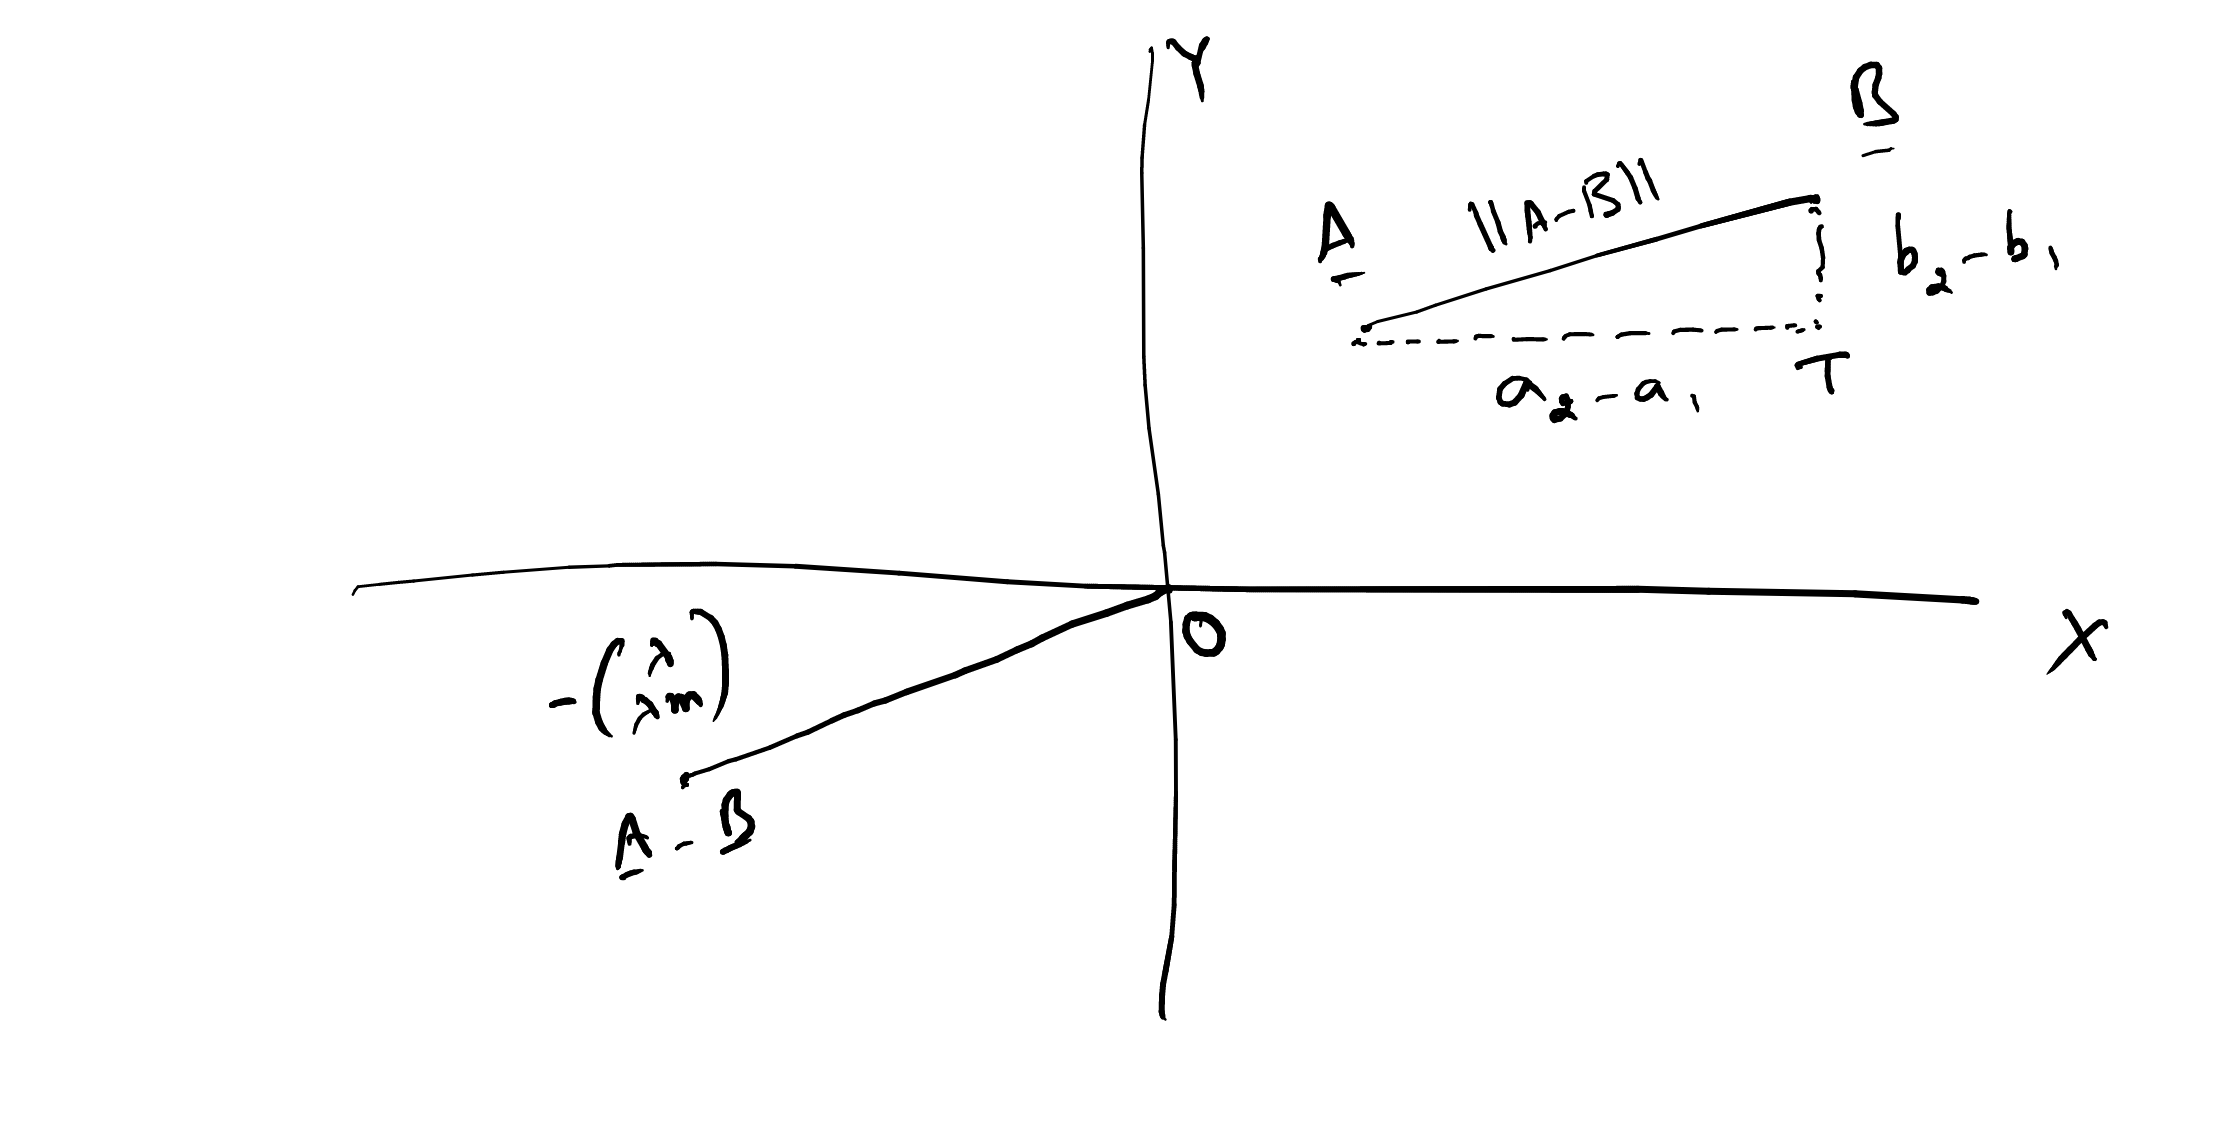
\includegraphics[width=\columnwidth]{./figs/ab.eps}
\caption{}
\label{fig:ab}
\end{figure}
%
\\
\solution See Fig. \ref{fig:ab}. From \eqref{eq:nhomog}, for some 
$\lambda$,
\begin{align}
\vec{B} &=\vec{A} + \lambda \myvec{1 \\ m}
\\
\implies \vec{A} - \vec{B} &= - \lambda \myvec{1 \\ m},
\end{align}
%
$\vec{A} - \vec{B}$ is marked in Fig. \ref{fig:ab}.
%
\item Show that $AB = \norm{\vec{A}-\vec{B}}$
\item Show that the equation of $AB$ is
\begin{align}
\label{eq:line_ab}
\vec{x} = \vec{A}+ \lambda\brak{\vec{B}-\vec{A}}
\end{align}

\end{enumerate}
%
\section{Orthogonality}
\begin{enumerate}[label=\thesection.\arabic*
,ref=\thesection.\theenumi]
\item See Fig. \ref{fig:orth}.  In $\triangle ABC, AB \perp BC$. Show that
\begin{equation}
\brak{\vec{A}-\vec{B}}^T\brak{\vec{B}-\vec{C}} = 0
\label{eq:orth}
\end{equation}
\begin{figure}
\centering
\includegraphics[width=\columnwidth]{./figs/orth.eps}
\caption{}
\label{fig:orth}
\end{figure}
%
\solution Using Baudhayana's theorem,
\begin{align}
\norm{\vec{A}-\vec{B}}^2 + \norm{\vec{B}-\vec{C}}^2 &= 
\norm{\vec{C}-\vec{A}}^2
\\
\implies 
\brak{\vec{A}-\vec{B}}^T\brak{\vec{A}-\vec{B}} 
&+ 
\brak{\vec{B}-\vec{C}}^T\brak{\vec{B}-\vec{C}} 
\nonumber \\
&= 
\brak{\vec{C}-\vec{A}}^T \brak{\vec{C}-\vec{A}}
\nonumber \\
\implies 
2\vec{A}^T\vec{B} - 2\vec{B}^T\vec{B}&+2\vec{B}^T\vec{C}-2\vec{A}^T\vec{C}
=0
\end{align}
which can be simplified to obtain \eqref{eq:orth}.
%
\item Let $\vec{x}$ be any point on $AB$ in Fi.g \ref{fig:orth}.  Show that
\begin{equation}
\brak{\vec{x}-\vec{A}}^T\brak{\vec{B}-\vec{C}} = 0
\end{equation}
%
\item If $\vec{x,y}$ are any two points on $AB$, show that 
\begin{equation}
\label{eq:orth_any}
\brak{\vec{x}-\vec{y}}^T\brak{\vec{B}-\vec{C}} = 0
\end{equation}
%
\item In Fig. \ref{fig:alt}, $BE \perp AC, CF \perp AB$.  Show that $AD \perp BC$.
\begin{figure}[!hb]
\centering
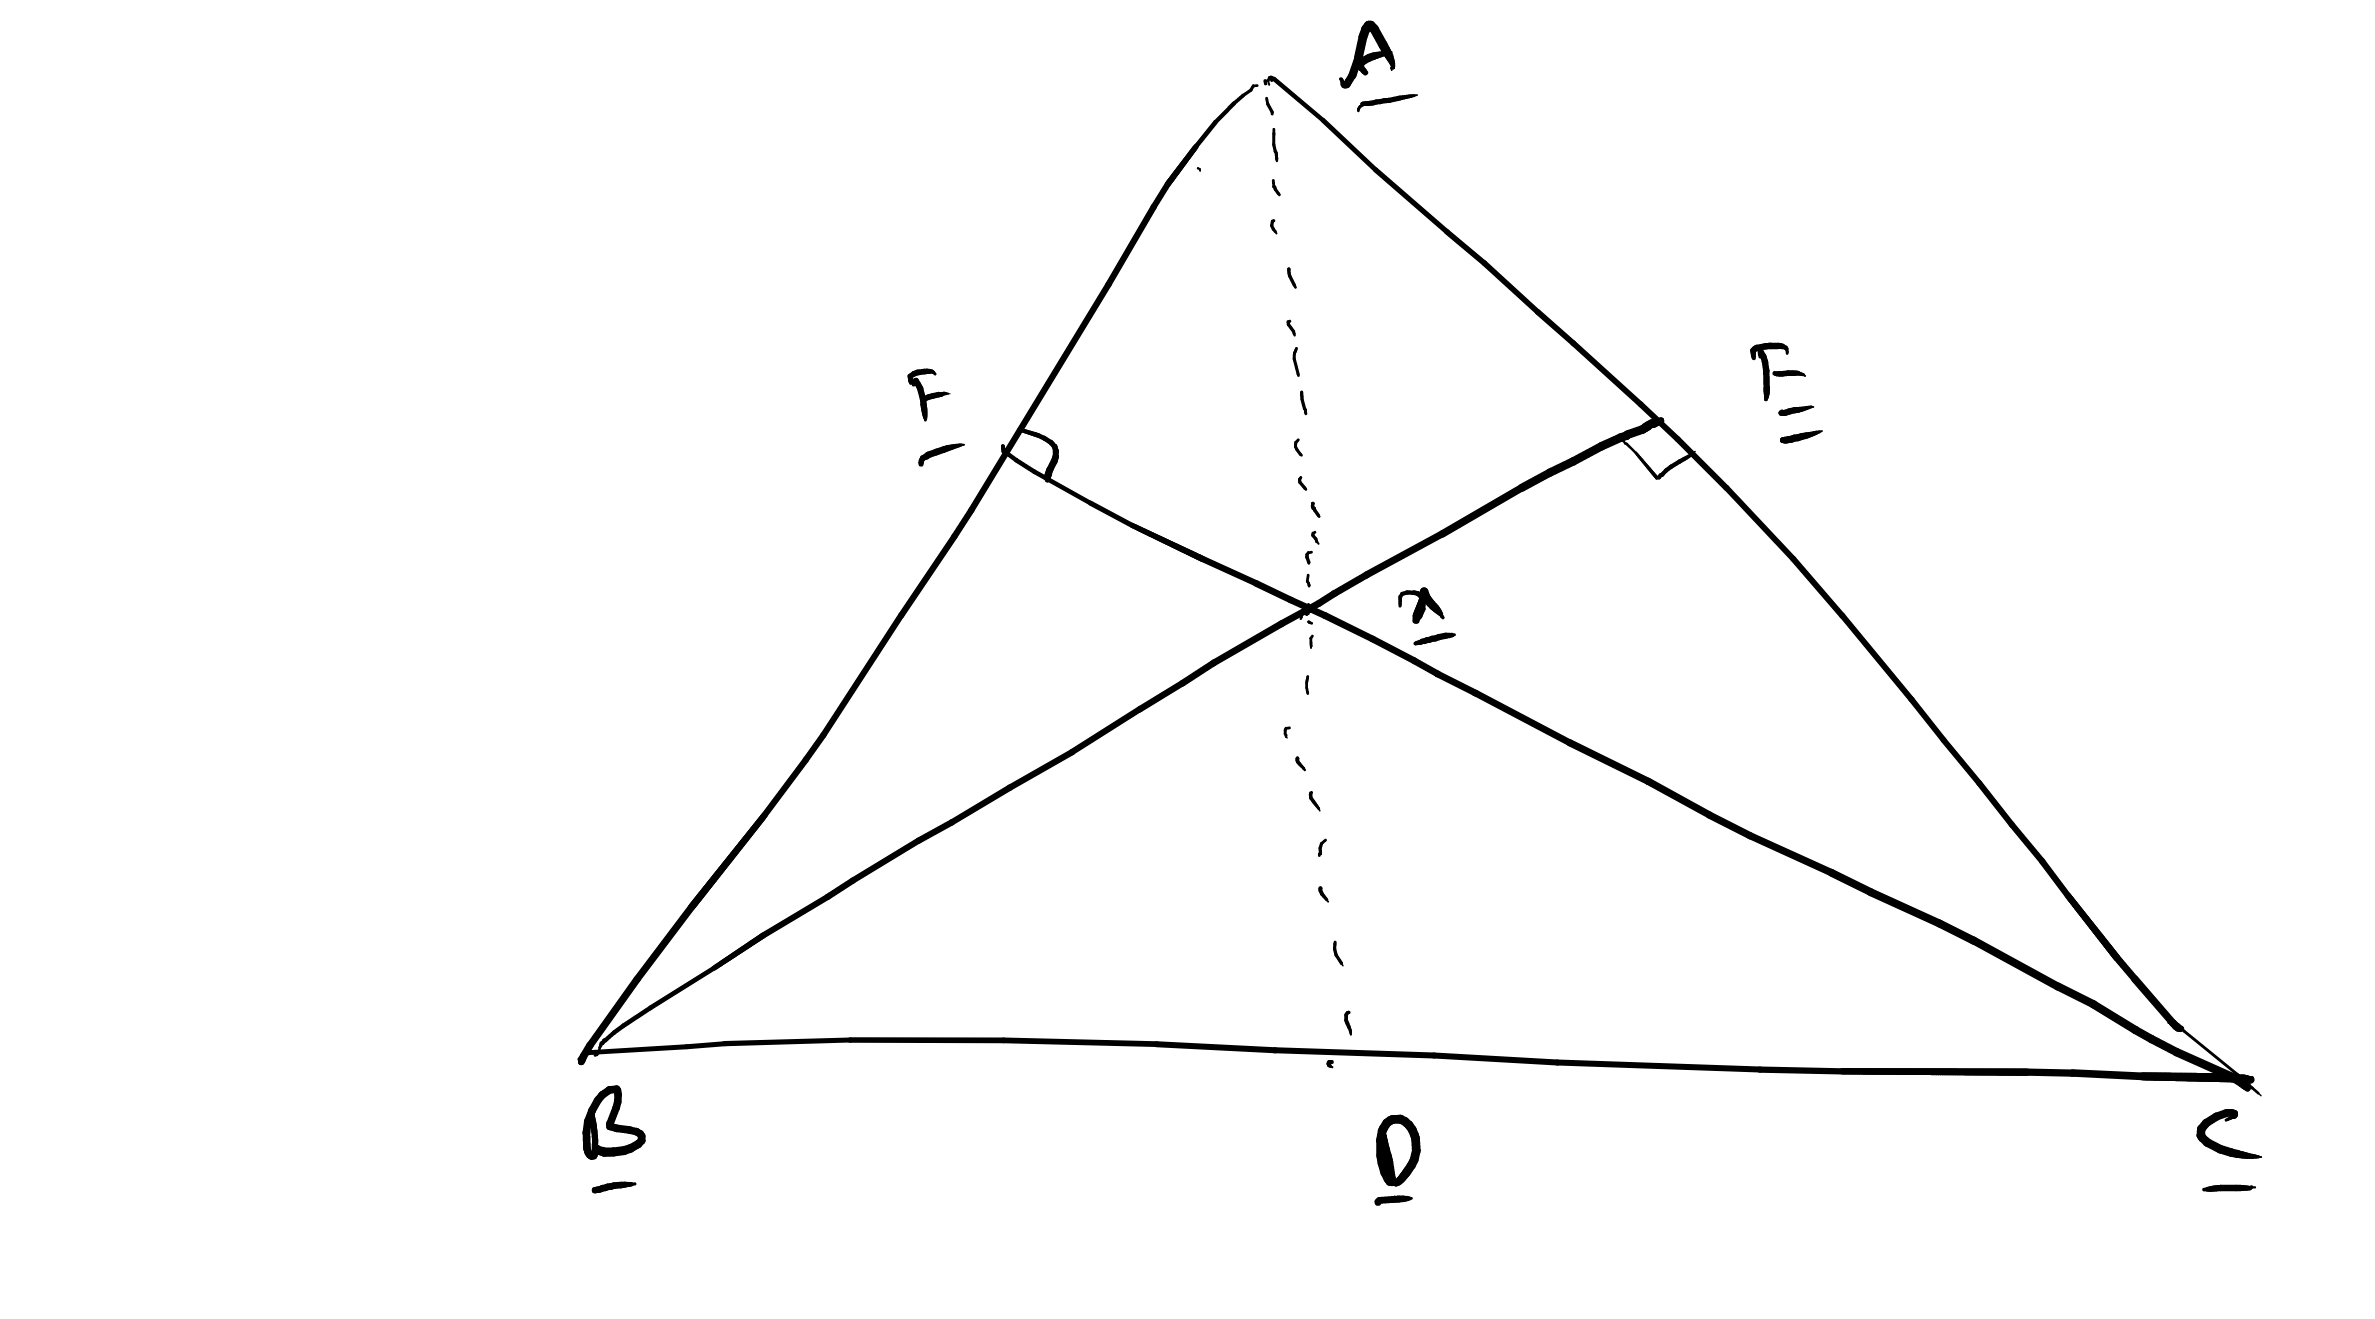
\includegraphics[width=\columnwidth]{./figs/alt.eps}
\caption{}
\label{fig:alt}
\end{figure}
\\
\solution Let $\vec{x}$ be the intersection of $BE$ and $CF$. Then, using 
\eqref{eq:orth_any},
\begin{align}
\label{eq:alt_1}
\begin{split}
\brak{\vec{x}-\vec{B}}^T
\brak{\vec{A}-\vec{C}} &= 0
\\
\brak{\vec{x}-\vec{C}}^T
\brak{\vec{A}-\vec{B}} &=0
\end{split}
\\
\label{eq:alt_3}
\implies \vec{x}^T\brak{\vec{A}-\vec{C}}-\vec{B}^T\brak{\vec{A}-\vec{C}} &= 0
\\
\text{and }\vec{x}^T\brak{\vec{A}-\vec{B}}-\vec{C}^T\brak{\vec{A}-\vec{B}} &= 0
\label{eq:alt_4}
\end{align}
%
Subtracting \eqref{eq:alt_4} from \eqref{eq:alt_3},
\begin{align}
\vec{x}^T\brak{\vec{B}-\vec{C}} + \vec{A}^T\brak{\vec{C}-\vec{B}} &= 0
\\
\implies \brak{\vec{x}^T - \vec{A}^T}\brak{\vec{B}-\vec{C}}  &= 0
\\
\implies \brak{\vec{x} - \vec{A}}^T\brak{\vec{B}-\vec{C}}  &= 0
\end{align}
%
which completes the proof.
\end{enumerate}
%
\section{Medians of a triangle}
\begin{enumerate}[label=\thesection.\arabic*
,ref=\thesection.\theenumi]
\item In Fig. \ref{fig:ratio},
\begin{equation}
\frac{AB}{BC} = \frac{\norm{\vec{A}-\vec{B}}}{\norm{\vec{B}-\vec{C}}} = k.
\label{eq:k}
\end{equation}
%
Show that
%
\begin{equation}
\frac{\vec{A}+k\vec{C}}{k+1} = \vec{B}.
\label{eq:ratio}
\end{equation}
%
\begin{figure}[!hb]
\centering
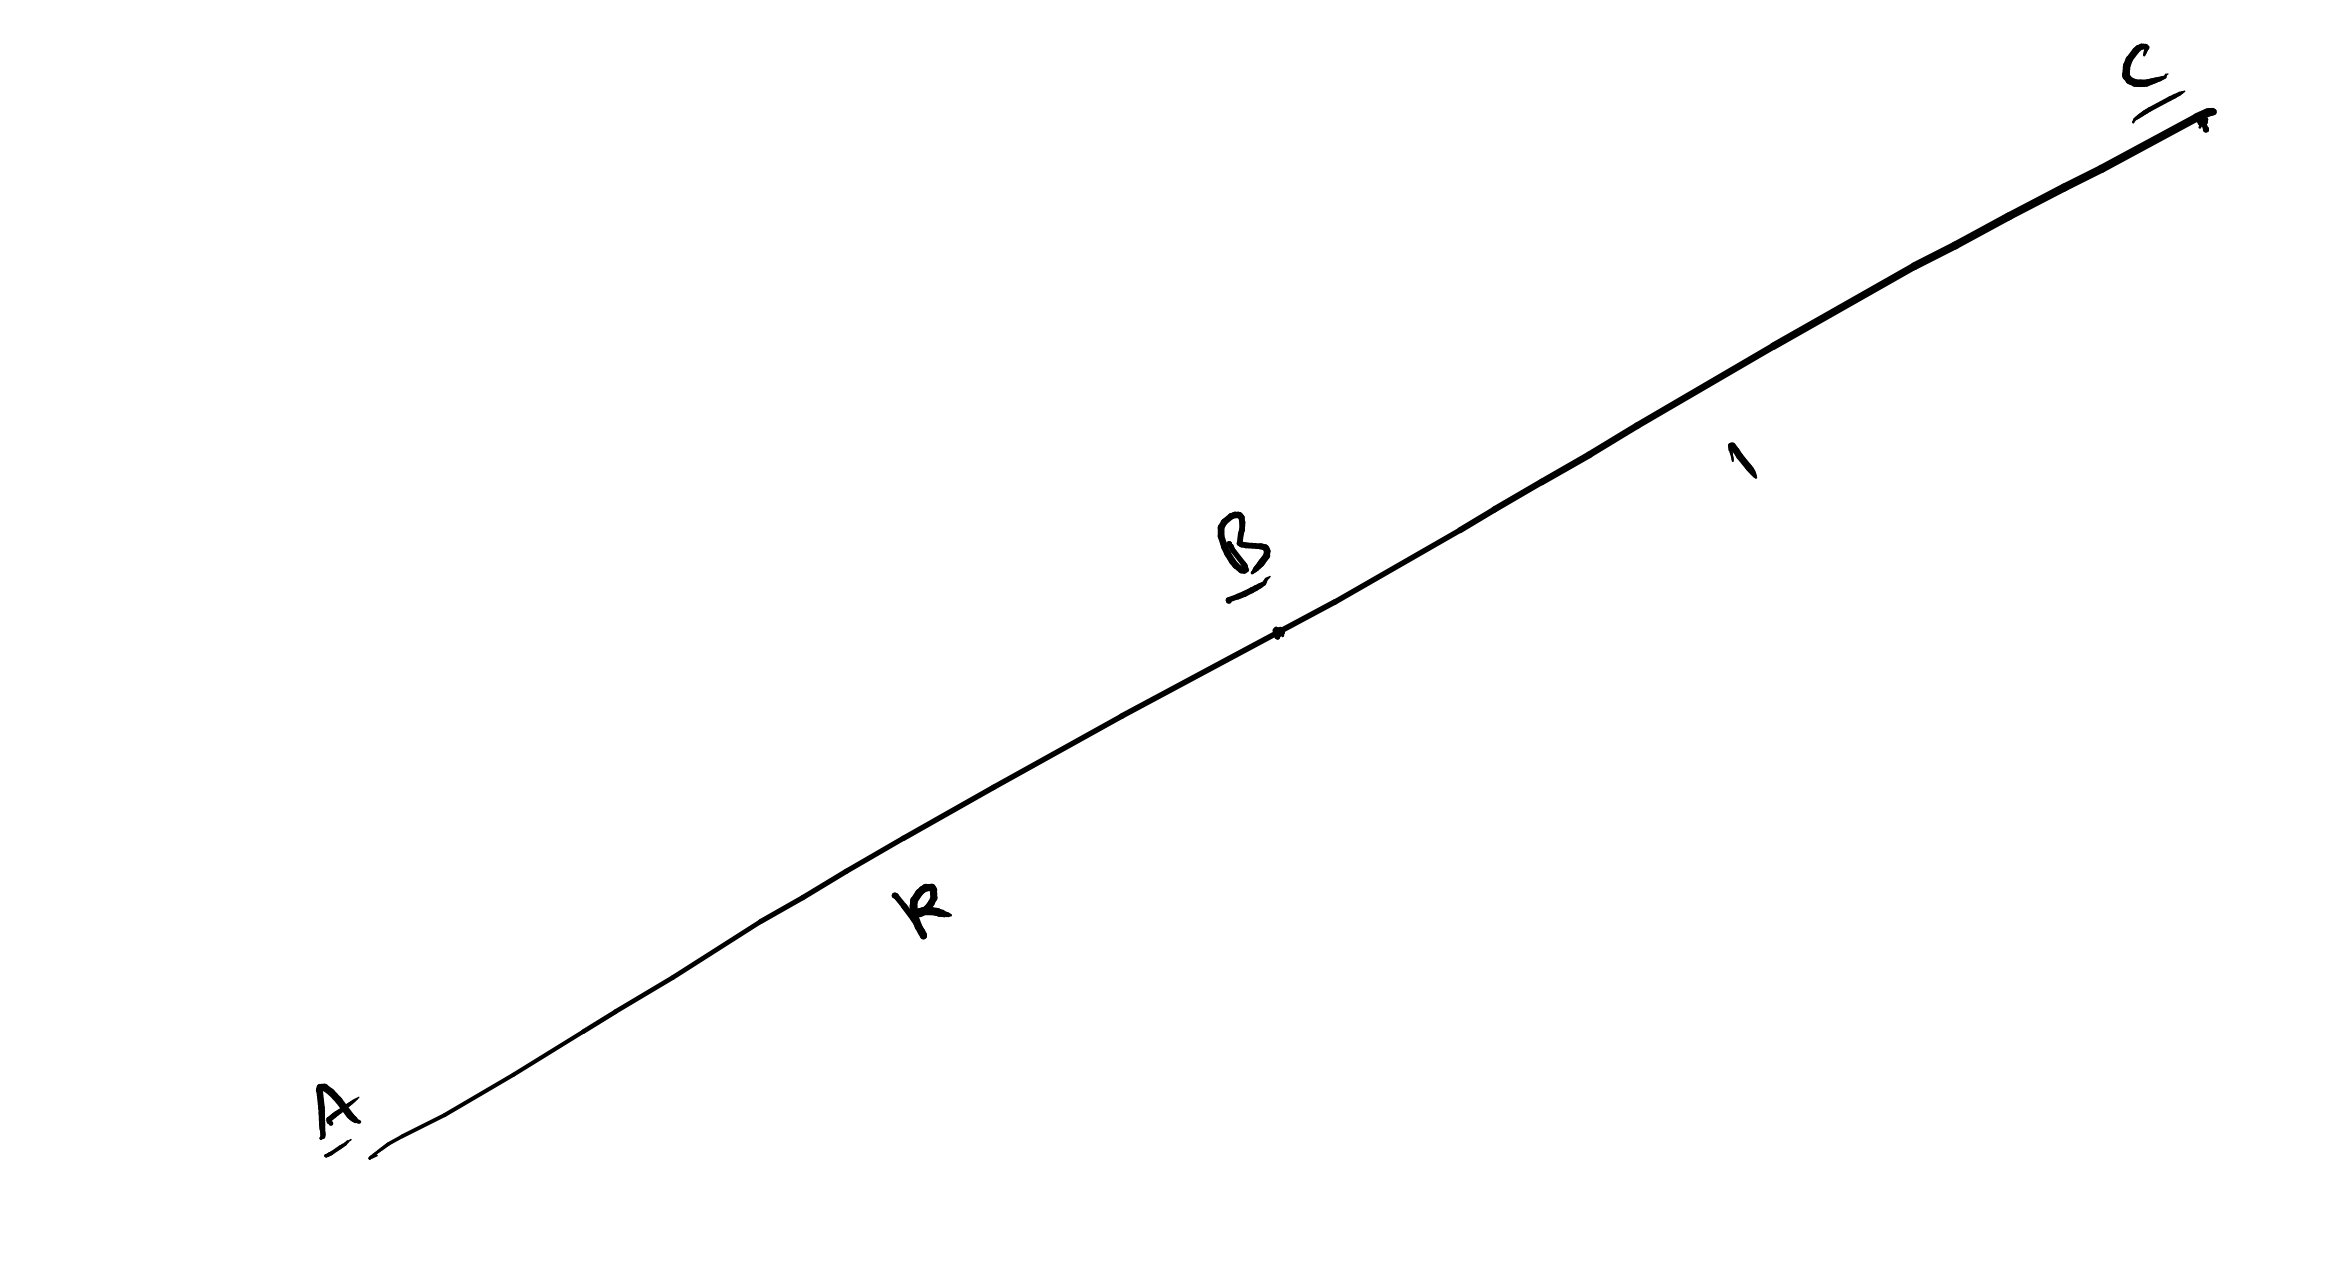
\includegraphics[width=\columnwidth]{./figs/ratio.eps}
\caption{}
\label{fig:ratio}
\end{figure}
\solution From \eqref{eq:nhomog}, 
\begin{align}
\begin{split}
\vec{B} &= \vec{A} + \lambda_1 \myvec{1 \\ m},
\\
\vec{B} &= \vec{C} - \lambda_2 \myvec{1 \\ m}.
\end{split}
\\
\label{eq:rat_1}
\implies \frac{\norm{\vec{A}-\vec{B}}}{\norm{\vec{B}-\vec{C}}} &= 
\frac{\lambda_1}{\lambda_2} = k
\\
\text{and } \frac{\vec{B}- \vec{A}}{\lambda_1} &= \frac{\vec{C}- 
\vec{B}}{\lambda_2} =  \myvec{1 \\ m},
\label{eq:rat_2}
\end{align}
%
from \eqref{eq:k}. Using \eqref{eq:rat_1} and \eqref{eq:rat_1},
\begin{align}
\vec{A}- \vec{B} &=  k\brak{\vec{B}- \vec{C}}
\end{align}
%
resulting in \eqref{eq:ratio}.
%
\item If $\vec{A}$ and $\vec{B}$ are linearly independent,  
\begin{equation}
k_1\vec{A} + k_2\vec{B} = 0 \implies k_1=k_2=0
\end{equation}
\item $BE$ and $CF$ are medians of $\triangle ABC$ intersecting at $O$ as shown in Fig. \ref{fig:median}. 
Show that
\begin{equation}
\frac{CO}{OF} = \frac{BO}{OE} = 2
\end{equation}
%
\begin{figure}[!hb]
\centering
\includegraphics[width=\columnwidth]{./figs/median.eps}
\caption{}
\label{fig:median}
\end{figure}
\solution Let
\begin{align}
\frac{CO}{OF} &= k_1
\\
\frac{BO}{OE} &= k_2
\end{align}
%
Using  \eqref{eq:ratio},
\begin{align}
\vec{E}&= \frac{\vec{A} + \vec{C}}{2}
\\
\vec{F}&= \frac{\vec{A} + \vec{B}}{2}
\end{align}
%
and
\begin{align}
\label{eq:o1}
\vec{O}&= \frac{k_1\vec{F} + \vec{C}}{k_1+1} = \frac{k_1\frac{\vec{A} + \vec{B}}{2} + \vec{C}}{k_1+1}
\\
\vec{O}&= \frac{k_2\vec{E} + \vec{B}}{k_2+1} = \frac{k_2\frac{\vec{A} + \vec{C}}{2} + \vec{B}}{k_2+1}
\label{eq:o2}
\end{align}
%
From \eqref{eq:o1} and \eqref{eq:o2},
\begin{align}
 \frac{k_1\frac{\vec{A} + \vec{B}}{2} + \vec{C}}{k_1+1} &= 
 \frac{k_2\frac{\vec{A} + \vec{C}}{2} + \vec{B}}{k_2+1}
\end{align}
\begin{multline}
\label{eq:lin_comb}
\implies \sbrak{\frac{k_1\brak{k_2+1}}{2}
-\frac{k_2\brak{k_1+1}}{2}}\vec{A} 
\\
+ 
\sbrak{\frac{k_1\brak{k_2+1}}{2}-\brak{k_1+1}}\vec{B} 
\\
+ \sbrak{\brak{k_2+1}-\frac{k_2\brak{k_1+1}}{2}}\vec{C} 
= 0
\end{multline}
resulting in $k_1 = k_2$,
\begin{align}
k_1^2-k_1-2  &= 0
\implies k_1 = k_2 = 2,
\end{align}
provided $\vec{A},\vec{B},\vec{C}$ are linearly independent. Thus, substituting $k_1=2$ in \eqref{eq:o2},
\begin{equation}
\vec{O} = \frac{\vec{A}+\vec{B}+\vec{C}}{3}
\end{equation}
%
If $\vec{A},\vec{B},\vec{C}$ are linearly dependent,
\begin{align}
\label{eq:lin_dep}
\vec{A} = \alpha \vec{B} + \beta \vec{C} 
\end{align}
%
Note that $\vec{B},\vec{C}$ are linearly independent.
Substituting \eqref{eq:lin_dep} in \eqref{eq:lin_comb},
\begin{multline}
%\label{eq:lin_comb}
 \sbrak{\frac{k_1\brak{k_2+1}}{2}
-\frac{k_2\brak{k_1+1}}{2}}\sbrak{\alpha \vec{B} + \beta \vec{C}  }
\\
+ 
\sbrak{\frac{k_1\brak{k_2+1}}{2}-\brak{k_1+1}}\vec{B} 
\\
+ \sbrak{\brak{k_2+1}-\frac{k_2\brak{k_1+1}}{2}}\vec{C} 
= 0
\end{multline}
\begin{align}
\implies
\begin{split}
\brak{k_1-k_2}\alpha + k_1k_2 - k_1-2 &=0
\\
\brak{k_1-k_2}\beta - k_1k_2 + k_2+2 &=0
\end{split}
\label{eq:median_contra}
\\
\implies \brak{k_1-k_2}\brak{\alpha +\beta - 1} = 0
\end{align}
If $\alpha+\beta = 1, \vec{A},\vec{B},\vec{C}$ are collinear according to \eqref{eq:ratio} resulting in a 
contradiction.  Hence, $k_1=k_2$, which, upon substitution in \eqref{eq:median_contra}, yields
\begin{equation}
k_1^2 - k_1-2 = 0 \implies k_1 = 2.
\end{equation}
\end{enumerate}
%
\section{Matrix Transformations}
\begin{enumerate}[label=\thesection.\arabic*
,ref=\thesection.\theenumi]

\item Find $\vec{R}$, the reflection  of $\vec{P}$ about the line
\begin{align}
L: \quad \vec{n}^T\vec{x} = c
\end{align}
%
\begin{figure}
\centering
\includegraphics[width=\columnwidth]{./figs/reflection.eps}
\caption{}
\label{fig:locus}
\end{figure}
\solution Since $\vec{R}$ is the reflection of $\vec{P}$ and $\vec{Q}$ lies on $L$, $\vec{Q}$ bisects $PR$.  
This leads to the following equations
Hence, 
\begin{align}
\label{eq:reflect_bisect}
2\vec{Q} &= \vec{P}+\vec{R}
\\
\label{eq:reflect_Q}
\vec{n}^{T}\vec{Q} &= c
\\
\label{eq:reflect_R}
\vec{m}^{T}\vec{R} &= \vec{m}^{T}\vec{P}
\end{align}
%
where $\vec{m}$ is the direction vector of $L$.  From \eqref{eq:reflect_bisect} and \eqref{eq:reflect_Q},
\begin{align}
\label{eq:reflect_bisectQ}
\vec{n}^{T}\vec{R}  &= 2c - \vec{n}^{T}\vec{P}
\end{align}
%
From \eqref{eq:reflect_bisectQ} and \eqref{eq:reflect_R},
\begin{align}
\label{eq:reflect_bisectQR}
\myvec{\vec{m} & \vec{n}}^T\vec{R} &= \myvec{\vec{m} & -\vec{n}}^T\vec{P}+ \myvec{0 \\ 2c}
\end{align}
%
Letting 
\begin{align}
\label{eq:reflect_mat}
\vec{V}=  \myvec{\vec{m} & \vec{n}}
\end{align}
with the condition that $\vec{m},\vec{n}$ are orthonormal, i.e.
\begin{align}
\label{eq:reflect_ortho}
\vec{V}^T\vec{V}=  \vec{I}
\end{align}
%
Noting that 
\begin{align}
\label{eq:reflect_trans}
\myvec{\vec{m} & -\vec{n}} &= \myvec{\vec{m} & \vec{n}} \myvec{1 & 0 \\ 0 & -1},
\end{align}
\eqref{eq:reflect_bisectQR} can be expressed as
%
\begin{align}
\label{eq:reflect_}
\vec{V}^T\vec{R} &=  \sbrak{\vec{V}\myvec{1 & 0 \\ 0 & -1}}^T\vec{P}+\myvec{0 \\ 2c}
\\
\implies \vec{R} &= \sbrak{\vec{V}\myvec{1 & 0 \\ 0 & -1}\vec{V}^{-1}}^T\vec{P}+ \vec{V}\myvec{0 \\ 2c}
\\
 &=\vec{V}\myvec{1 & 0 \\ 0 & -1}\vec{V}^T \vec{P}+2c \vec{n}
\end{align}

\item Rotate $\vec{P}$ through an angle of  $ \theta $  about the origin in the counter clockwise 
direction to obtain $\vec{S}$.
\\
\solution 
\begin{align}
\label{eq:rotate}
\vec{S} &= \myvec{\cos \theta & -\sin \theta \\ \sin \theta & \cos \theta} \vec{P}
\end{align}


\end{enumerate}


\section{Circumcircle}
\begin{enumerate}[label=\thesection.\arabic*
,ref=\thesection.\theenumi]
\item A circle with centre at  $\vec{O}$ and radius $r$ has the equation 
\begin{align}
\norm{\vec{x}-\vec{O}}&=r
\\
\implies \brak{\vec{x}-\vec{O}}^T\brak{\vec{x}-\vec{O}} &= r^2
\label{eq:circle}
\end{align}
\item Let $\vec{A},\vec{B}$ and $\vec{C}$ be three points on the circle and 
$D$ be a point on $BC$ such that
$OD \perp BC$ as in Fig. \ref{fig:ccircle}.  Show that 
\begin{align}
\vec{D}=\frac{\vec{B}+\vec{C}}{2}
\end{align}
%
\begin{figure}[!ht]
	\begin{center}
		
		%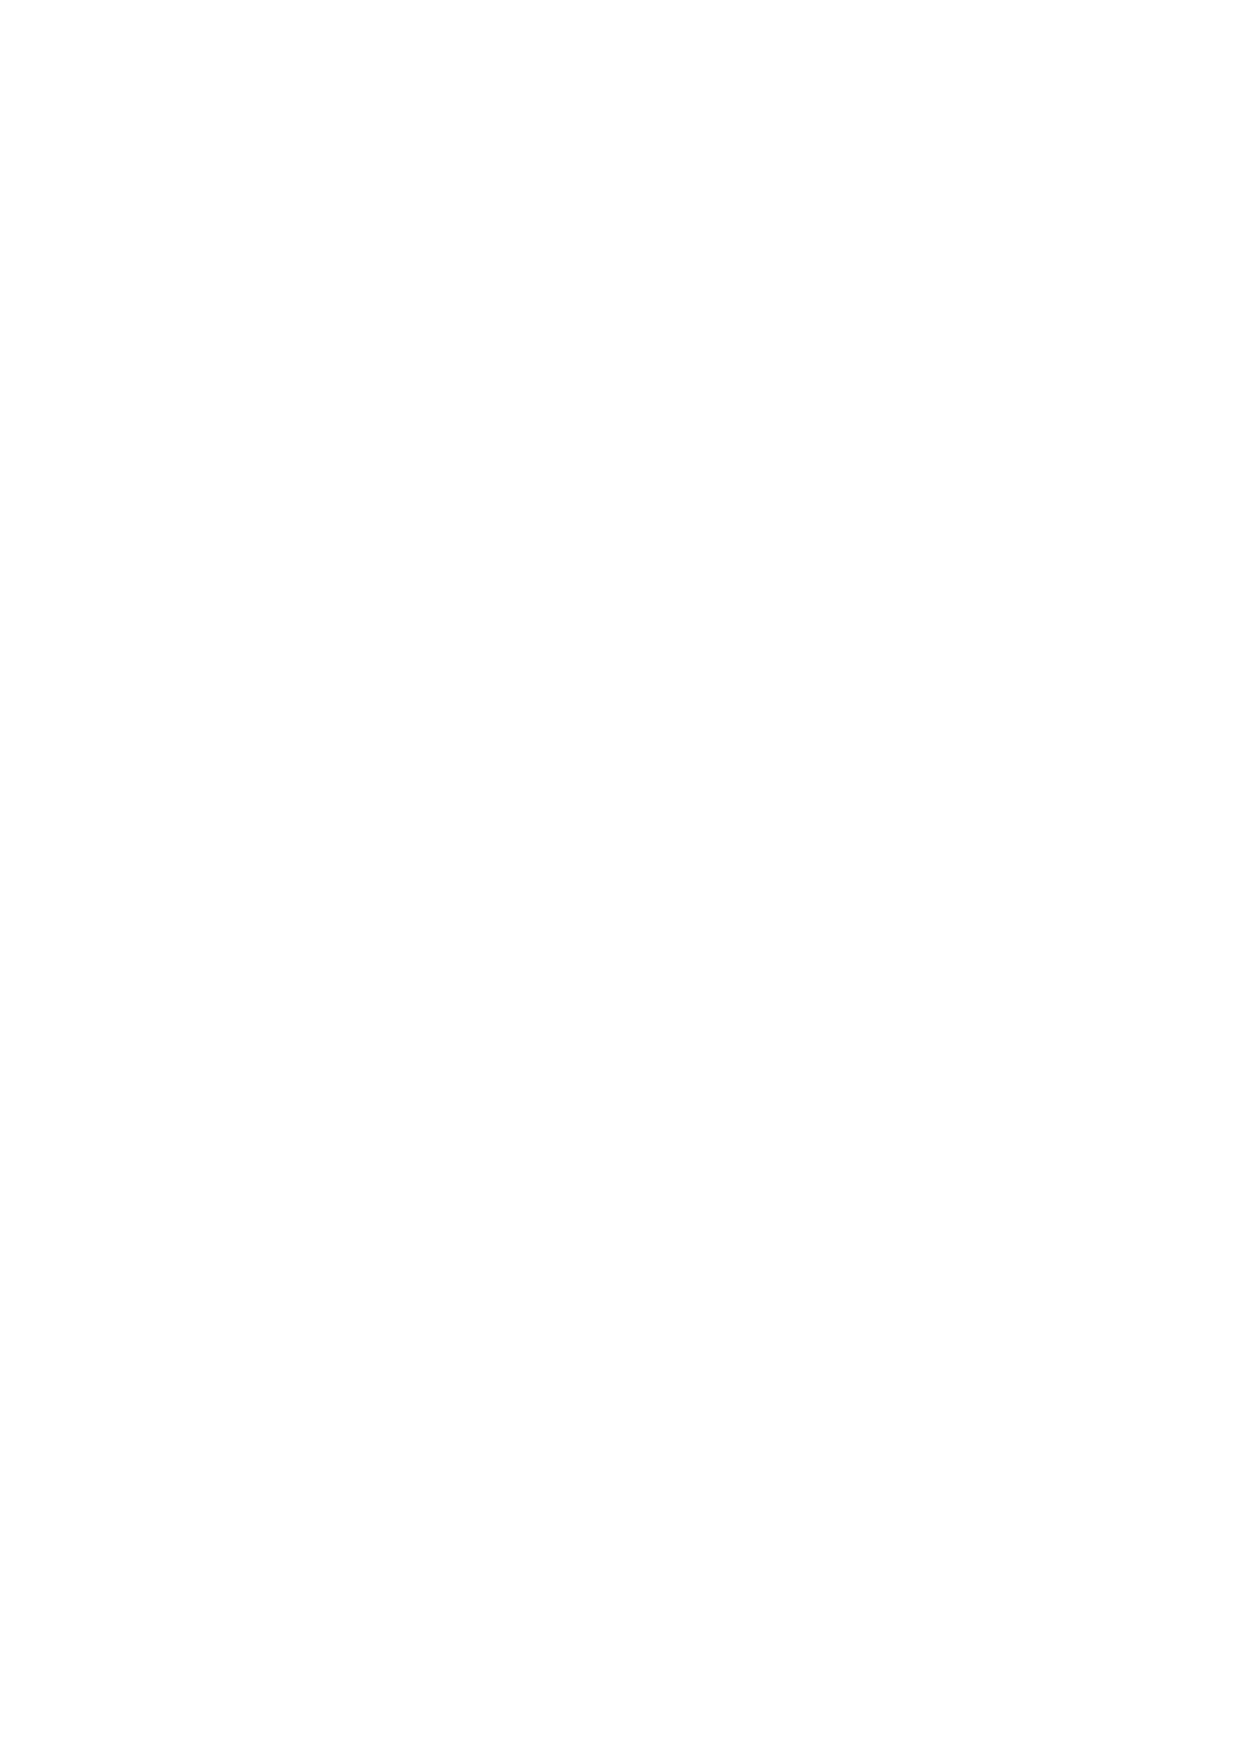
\includegraphics[width=\columnwidth]{./figs/ch3_angle_bisector}
		%\vspace*{-10cm}
		\resizebox{\columnwidth}{!}{\begin{tikzpicture}
[scale=2,>=stealth,point/.style={draw,circle,fill = black,inner sep=0.5pt},]

%\node (D) at (0, 0)[point,label=below :$D$] {};
\node (B) at (-2, -2)[point,label=below left :$B$]{};
\node (A) at (1, 3)[point,label=above:$A$]{};
\node (C) at (4, -1)[point,label=below right:$C$]{};
%\coordinate [point, label={above : $O$ }] (I) at  (1.147, 1.143);
\node (O) at (0.7962963,-0.27777778)[point,label=above:$O$]{};
\node (D) at ( 1,-1.5)[point,label=below:$D$]{};
%\node (x1) at (0.601,-1.357)[point,label=left:$x_1$]{};
%\node (x2) at (2.15,-1.1)[point,label=right:$x_2$]{};
%\node (temp) at ($(O)!0.5!(D)$)[label=right:$r$]{};
%\node (D) at (2.424,1.1)[point,label=above right:$D$]{};
%\node (E) at (1.1, 1.9)[point,label=above right:$E$]{};
%\node (F) at (-1.1, 1.9)[point,label=above left:$F$]{};
\def\rad{3.284101453883}
\draw (O) circle (\rad);

\draw (D)--(O);
\draw (A)--(B);
\draw (B)--(C);
\draw (A)--(C);
%\draw (C)--(D);
%\draw [thick,dashed] (x1) -- (x2);
%\draw [thick,dashed] (O) -- (E);
%\draw [thick,dashed] (O) -- (F);
%\draw (B)--(O);
%\draw (C)--(O);

%\tkzMarkRightAngle[size=.2](A,D,C)
%\tkzMarkRightAngle[size=.15](B,F,O);
%\tkzMarkRightAngle[size=.15](C,E,O);
%\tkzMarkAngle[size=.4](D,B,O);
%\tkzMarkAngle[size=.35](O,B,F);
%\tkzMarkAngle[size=.54](E,C,O);
%\tkzMarkAngle[size=.5](E,C,O);
%\tkzMarkAngle[size=.6](O,C,D);
%\tkzMarkAngle[size=.65](O,C,D);

\end{tikzpicture}}
	\end{center}
	\caption{Circumcircle.}
	\label{fig:ccircle}	
\end{figure}


\solution From \eqref{eq:circle},
\begin{align}
\norm{\vec{B}-\vec{O}}^2=\norm{\vec{C}-\vec{O}}^2=r^2
\\
 \implies \brak{\vec{B}-\vec{O}}^T\brak{\vec{B}-\vec{O}} = 
\brak{\vec{C}-\vec{O}}^T\brak{\vec{C}-\vec{O}} 
\\
 \implies \brak{\vec{B}-\vec{C}}^T\brak{\frac{\vec{B}+\vec{C}}{2} - 
\vec{O}}  = 0
\label{eq:circle_mid}
\end{align}
after simplification. Since $OD \perp BC$,
\begin{align}
\brak{\vec{B}-\vec{C}}^T\brak{\vec{D}-\vec{O}} = 0 
\label{eq:circle_D}
\end{align}
Since $D$ and $\frac{\vec{B}+\vec{C}}{2}$ lie on $BC$, using 
\eqref{eq:line_ab},
\begin{align}
\label{eq:circle_mid_D1}
\frac{\vec{B}+\vec{C}}{2}
&= \vec{B}+ \lambda_1\brak{\vec{B}-\vec{C}}
\\
\vec{D}
&= \vec{B}+ \lambda_2\brak{\vec{B}-\vec{C}}
\label{eq:circle_mid_D2}
\end{align}
Multiplying \eqref{eq:circle_mid_D1} and \eqref{eq:circle_mid_D2} with 
$\brak{\vec{B}-\vec{C}}^T$ and subtracting, $\lambda_1=\lambda_2$
%
\begin{align}
\implies \vec{D} = \frac{\vec{B}+\vec{C}}{2}
\label{eq:circle_bisect}
\end{align}
%
\item Let  $\vec{D}$ be the mid point of $BC$.  Show that $OD \perp BC$.
%
\end{enumerate}


\section{Incircle}
\begin{enumerate}[label=\thesection.\arabic*
,ref=\thesection.\theenumi]
\item The circle with centre $\vec{O}$ and radius $r$ in Fig.\ref{fig:ang_bisect}	
 is inside 
$\triangle ABC$ and touches $AB, BC$ 
and $CA$ at $\vec{F}, \vec{D}$ and $\vec{E}$ respectively. $AB, BC$ and 
$CA$ are known as {\em tangents} to the circle.
\begin{figure}[!ht]
	\begin{center}
		
		%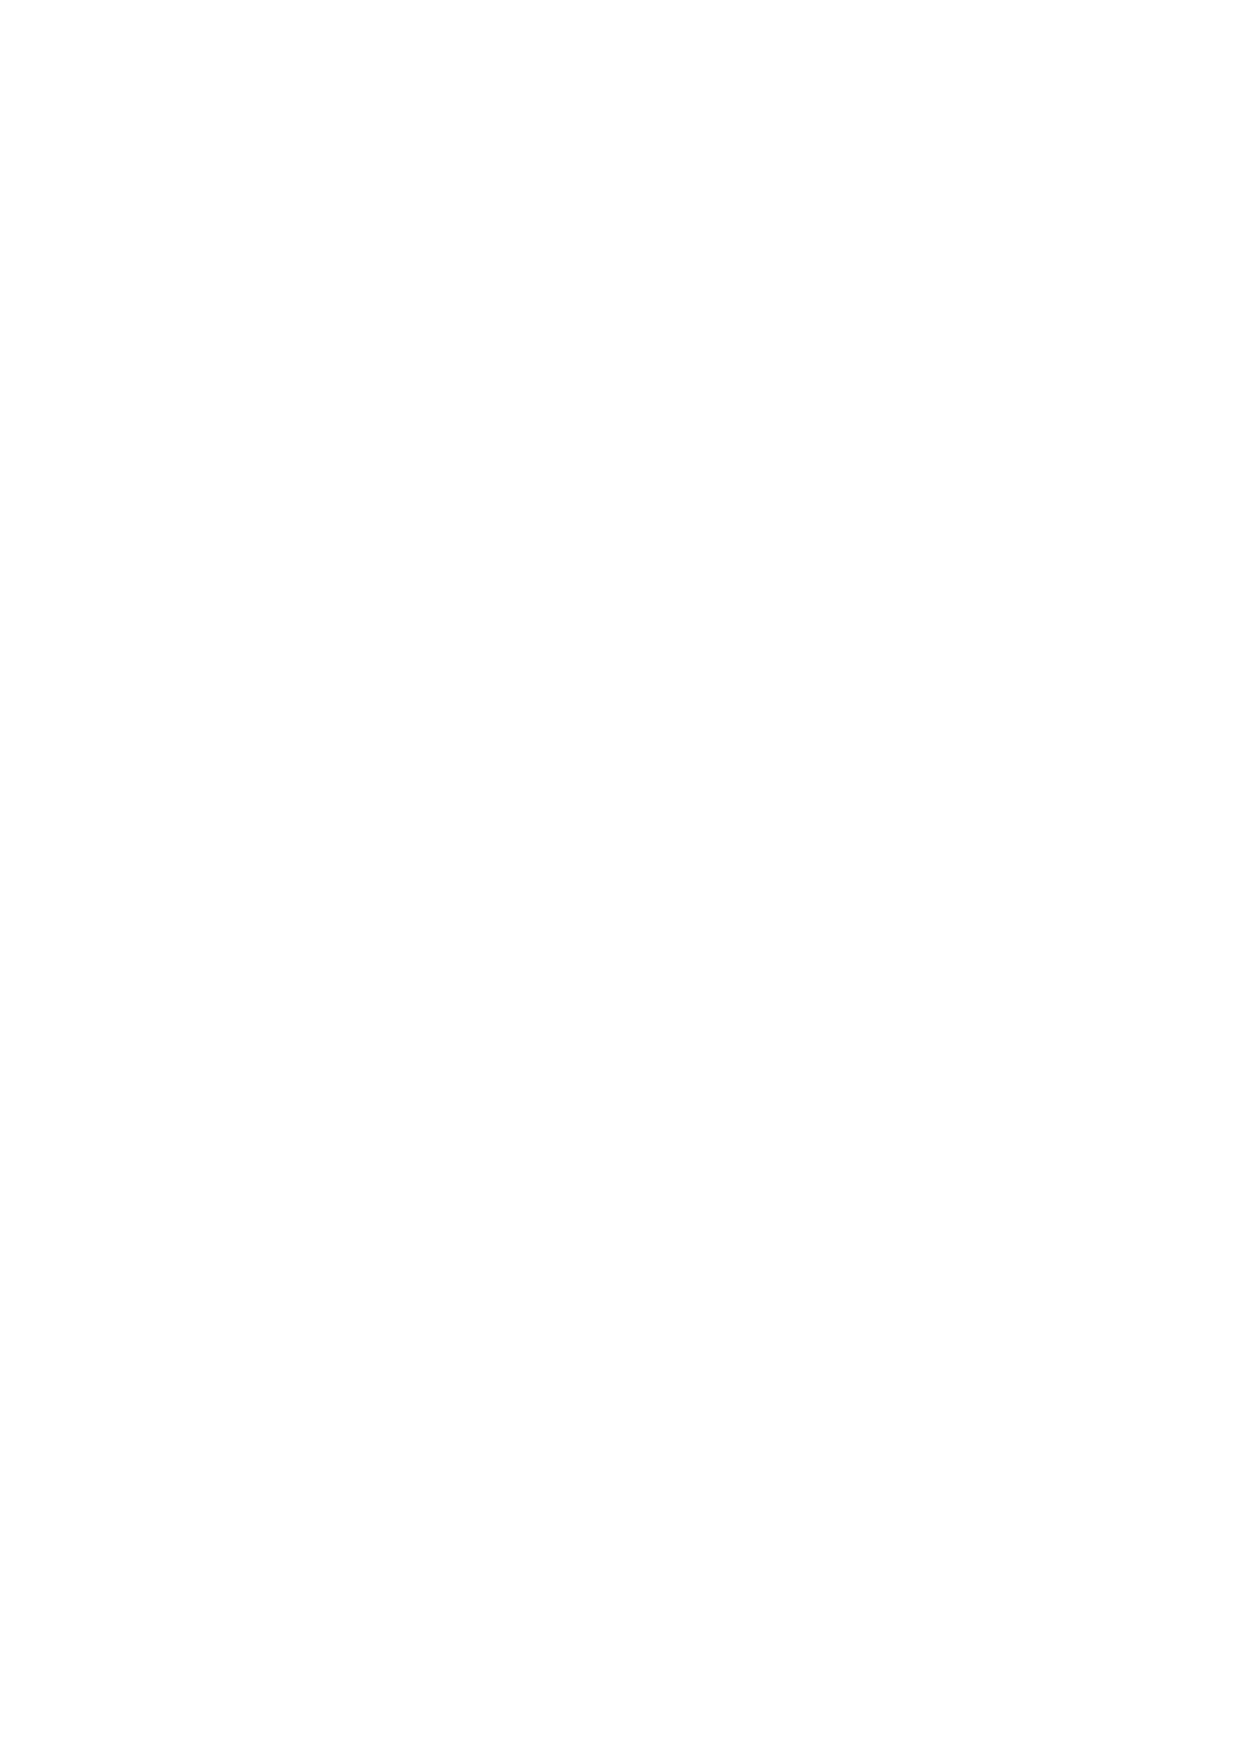
\includegraphics[width=\columnwidth]{./figs/ch3_angle_bisector}
		%\vspace*{-10cm}
		\resizebox{\columnwidth}{!}{\begin{tikzpicture}
[scale=2,>=stealth,point/.style={draw,circle,fill = black,inner sep=0.5pt},]

%\node (D) at (0, 0)[point,label=below :$D$] {};
\node (B) at (-2, -2)[point,label=below left :$B$]{};
\node (A) at (1, 3)[point,label=above:$A$]{};
\node (C) at (4, -1)[point,label=below right:$C$]{};
%\coordinate [point, label={above : $O$ }] (I) at  (1.147, 1.143);
\node (O) at (1.147, 0.143)[point,label=above:$I$]{};
\node (D) at (1.41,-1.43)[point,label=below:$U$]{};
\node (x1) at (0.601,-1.357)[point,label=left:$x_1$]{};
\node (x2) at (2.15,-1.1)[point,label=right:$x_2$]{};
\node (temp) at ($(O)!0.5!(D)$)[label=right:$r$]{};
%\node (D) at (2.424,1.1)[point,label=above right:$D$]{};
%\node (E) at (1.1, 1.9)[point,label=above right:$E$]{};
%\node (F) at (-1.1, 1.9)[point,label=above left:$F$]{};
\def\rad{1.596}
\draw (O) circle (\rad);

\draw (D)--(O);
\draw (A)--(B);
\draw (B)--(C);
\draw (A)--(C);
%\draw (C)--(D);
\draw [thick,dashed] (x1) -- (x2);
%\draw [thick,dashed] (O) -- (E);
%\draw [thick,dashed] (O) -- (F);
%\draw (B)--(O);
%\draw (C)--(O);

%\tkzMarkRightAngle[size=.2](A,D,C)
%\tkzMarkRightAngle[size=.15](B,F,O);
%\tkzMarkRightAngle[size=.15](C,E,O);
%\tkzMarkAngle[size=.4](D,B,O);
%\tkzMarkAngle[size=.35](O,B,F);
%\tkzMarkAngle[size=.54](E,C,O);
%\tkzMarkAngle[size=.5](E,C,O);
%\tkzMarkAngle[size=.6](O,C,D);
%\tkzMarkAngle[size=.65](O,C,D);

\end{tikzpicture}
}
	\end{center}
	\caption{Tangent and incircle.}
	\label{fig:ang_bisect}	
\end{figure}


\item Show that $OD \perp BC$.
%\begin{figure}[!h]
%\centering
%\resizebox {\columnwidth} {!} {
%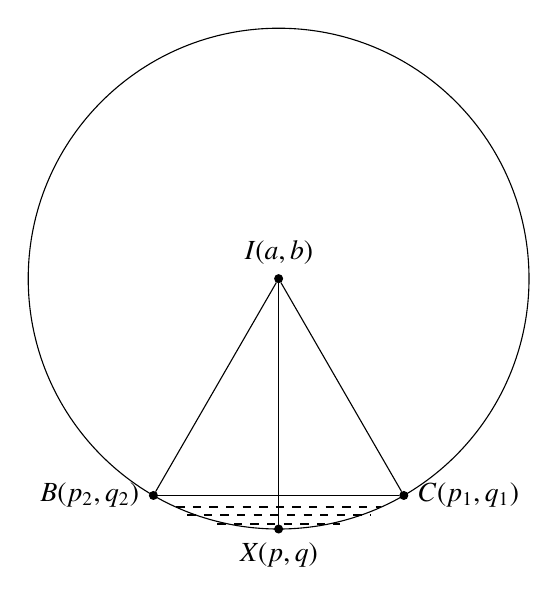
\begin{tikzpicture}
[
scale =2,
>=stealth,
point/.style = {draw, circle, fill = black, inner sep = 1pt},
]

\def\rad{1.59}
\coordinate [point, label={above : $I{(a,b)}$ }] (I) at (0, 0);
\draw (I) circle (\rad);

\node (C) at (300:{\rad})[point,label = right:$C{(p_1,q_1)}$] {};

\node (X) at (270:{\rad}) [point,label = below:$X{(p,q)}$] {};

\node (B) at (240:{\rad}) [point,label = left:$B{(p_2,q_2)}$] {};

\draw (C) -- (I);
\draw (B) -- (I);
\draw (B) -- (C);
\draw (I) -- (X);

\draw[black,thick,dashed](-0.65,-1.45) -- (0.65,-1.45);
\draw[black,thick,dashed](-0.58,-1.5) -- (0.58,-1.5);
\draw[black,thick,dashed](-0.39,-1.56) -- (0.39,-1.56);
\end{tikzpicture}

%}
%\caption{Notion of the derivative.}
%\label{fig:derivative}
%\end{figure}
\\
\solution Let $\vec{x}_1,\vec{x}_2$ be two points on the circle such that 
$x_1x_2 \parallel BC$. Then
%
\begin{align}
\norm{\vec{x}_1-\vec{O}}^2- 
\norm{\vec{x}_2-\vec{O}}^2 &= 0 
\\
\implies 
\brak{\vec{x}_1-\vec{x}_2}^T\brak{\frac{\vec{x}_1+\vec{x}_2}{2}-\vec{O}} &= 
0 
\\
\implies 
\brak{\vec{B}-\vec{C}}^T\brak{\frac{\vec{x}_1+\vec{x}_2}{2}-\vec{O}} &= 
0 
%\label{eq:circle_bisect}
\end{align}
%
For $\vec{x}_1=\vec{x}_2=\vec{D}$, $x_1x_2$ merges into $BC$ and the above 
equation becomes 
%
\begin{align}
\brak{\vec{B}-\vec{C}}^T\brak{\vec{D}-\vec{O}} = 
0 
\implies OD \perp BC
%\label{eq:circle_bisect}
\end{align}
%
\item Give an alternative proof for the above.
\\
\solution Let 
\begin{align}
\vec{B} & = \mbf{0}
\\
\vec{D} &= \lambda \vec{m}
\end{align}
Then
\begin{align}
\norm{\vec{D} - \vec{O}}^2 = r^2 &
\\
\implies \lambda^2\norm{\vec{m}}^2 - 2\lambda\vec{m}^T\vec{O} + \norm{\vec{O}}^2 &= r^2 
\end{align}
Since the above equation has a single root,
\begin{align}
\lambda = \frac{\vec{m}^T\vec{O}}{\norm{\vec{m}}^2}
\label{eq:incircle_lam}
\end{align}
%
Thus, 
\begin{align}
\brak{\vec{D} - \vec{B}}^T\brak{\vec{D} - \vec{O}}
&= \brak{\lambda\vec{m}}^T
\brak{\lambda\vec{m}-\vec{O}}
\\
&=\lambda^2\norm{\vec{m}}^2-\lambda\vec{m}^T\vec{O}
\\
&= \mbf{O} \text{ (from \ref{eq:incircle_lam})}.
\\
\implies & OD \perp BC
\end{align}
\item Find the equation of the tangent at $\vec{D}$.
\\
\solution The equation of the tangent is given by 
\begin{align}
\brak{\vec{O}-\vec{D}}^T\brak{\vec{x}-\vec{D}}=0
%\label{eq:circle_bisect}
\end{align}

\end{enumerate}
\section{Miscellaneous}
\begin{enumerate}[label=\thesection.\arabic*
,ref=\thesection.\theenumi]
%
\item Show that the angle in a semi-circle is a right angle.
\begin{figure}[!h]
\centering
\resizebox {\columnwidth} {!} {
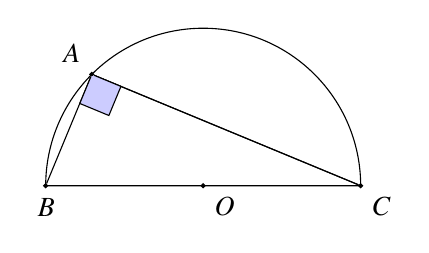
\begin{tikzpicture}
  [
    scale=2,
    >=stealth,
    point/.style = {draw, circle,  fill = black, inner sep = 0.5pt},
    dot/.style   = {draw, circle,  fill = black, inner sep = .2pt},
  ]

 \coordinate [point, label={below :	$B$ }] (B) at (-1, 0);
 \coordinate [point, label={below right:	$O$ }] (O) at (0, 0);
 \coordinate [point, label={below right:	$C$ }] (C) at (1, 0); 
 \coordinate [point, label={above left:	$A$ }] (A) at (-0.707,0.707);  
\draw (A) -- (C) arc(0:180:1) --cycle;
  \draw 
  (A) -- (B)
  (A) -- (C);
  \tkzMarkRightAngle[fill=blue!20,size=.2](B,A,C)    
%  \def\rad{1}

%  \draw (O) circle (\rad);  
%    \node (A) at +(45:{\rad}) [point,label = above right:$A$ $\brak{x,y}$] {};  
%  \path
%     (O)    edge  node[sloped, anchor=center, below, text width=0.5cm] { $r$}     (A) ; 
    
% \coordinate [point, label={below left:$B$}] (B) at (0, 0);
%    \node (A) at +(60:{2*sqrt(3)}) [label = above:$A$] {};
%  \coordinate [ label={below right:$C$ }] (C) at ($ (3,0) + sqrt(3)*(1,0) $);
%    \node (P) at +(30:{2*sqrt(3)}) [label = above:$P$] {};  
%  \path[->]
%     (B)    edge  node[sloped, anchor=center, below, text width=2.0cm] { $y = m_1x+c_1$}     (A) 
%	 (B)    edge  node[sloped, anchor=east, below, text width=2.0cm] { $y=m_2x+c_2$}     (C)
%	 (B)    edge  node[sloped, anchor=east, below, text width=2.0cm] { Bisector}     (P);
%  
%%  
%%  \coordinate [point, label={below left:$B$ $\brak{0,0}$}] (B) at (0, 0);
%%    \node (A) at +(60:{2*sqrt(3)}) [point, label = above:$A$ $\brak{a,b}$] {};
%%  \coordinate [point, label={below right:$C$ $\brak{c,0}$}] (C) at ($ (3,0) + sqrt(3)*(1,0) $);
%%  \node (D) at ({sqrt(3)},0) [point, label = below:$D$ $\brak{a,0}$] {};
%%    \node (E) at +(45:{(3+sqrt(3))/sqrt(2)}) [point, label = above right:$E$] {};
%%    \node (O) at +(45:{sqrt(6)}) [point, label = right:$O$] {};    
%%    \node (F) at +(60:{(3+sqrt(3))/2}) [point, label = left:$F$] {};        
%  \draw  (A) -- (B) -- (C);% -- (A);
%%  \node (D) at ($(B)!0.5!(C)$) [point, label = {below:$D$}]{};
%%  \draw (A) -- (D);  
%%  \draw (B) -- (E);    
%%  \draw[dashed] (C) -- (F);      
%\tkzMarkAngle[draw = black, fill = white, opacity=1](P,B,A)
%\tkzLabelAngle[pos = 0.8](P,B,A){$\theta$}
%\tkzMarkAngle[draw = black, fill = white, opacity=1,size=1.1](C,B,P)
%\tkzLabelAngle[pos = 0.9](C,B,P){$\theta$}

%\tkzMarkAngle[size=1.4,draw = black, fill = white, opacity=1](C,B,P)
%\tkzLabelAngle[pos=1.15,font=\scriptsize](C,B,P){$\theta$}

%  \tkzMarkAngle[fill=white,opacity=1,size=0.2,label={$\theta$},pos=0.2](P,B,A)  
%  \tkzMarkAngle[fill=blue!20,size=.4,label={$\theta$}](P,B,A)
%  \tkzMarkAngle[fill=blue!20,size=.2,label={$\theta$](C,B,P)
%  \tkzMarkRightAngle[fill=blue!20,size=.2](B,E,A)  
%  \path
%     (B)    edge  node[sloped, anchor=center, below, text width=2.0cm] { $k_1:1$}     (E)  
%	 (C)    edge  node[sloped, anchor=east, below, text width=2.0cm] { $1:k_2$}     (F);

\end{tikzpicture}


}
\caption{The straight line.}
\label{fig:ch2_line}
\end{figure}
\solution Let 
\begin{align}
\vec{O} = 0
\end{align}
From the given information,
\begin{align}
\label{eq:semi_circ_pt}
\norm{\vec{A}}^2 = \norm{\vec{B}}^2 = \norm{\vec{C}}^2 = r^2
\\
\norm{\vec{B}-\vec{C}}^2 =  \brak{2r}^2
\\
\vec{B} + \vec{C} = 0
\label{eq:semcirc_mid}
\end{align}
%
where $r$ is the radius of the circle. Thus,
\begin{multline}
\norm{\vec{A}-\vec{B}}^2 + \norm{\vec{A}-\vec{C}}^2 = 
2\norm{\vec{A}}^2 + \norm{\vec{B}}^2 + \norm{\vec{C}}^2
\\
-2\vec{A}^T\brak{\vec{B}+\vec{C}}
%\\
%\norm{\vec{B}-\vec{C}}^2 =  \brak{2r}^2
%\\
%\vec{B} + \vec{C} = 0
\end{multline}
From \eqref{eq:semcirc_mid} and \eqref{eq:semi_circ_pt},
\begin{multline}
\norm{\vec{A}-\vec{B}}^2 + \norm{\vec{A}-\vec{C}}^2 = 4r^2 = \norm{\vec{B}-\vec{C}}^2 
%\\
%\norm{\vec{B}-\vec{C}}^2 =  \brak{2r}^2
%\\
%\vec{B} + \vec{C} = 0
\end{multline}
Thus, using Baudhayana's theorem, $\triangle ABC$ is right angled.
\item 	Show that $PA.PB = PC^2$, where $PC$ is the tangent to the circle in Fig. \ref{fig:tangent_secant}.

	\begin{figure}[!hb]
		\begin{center}
			
			%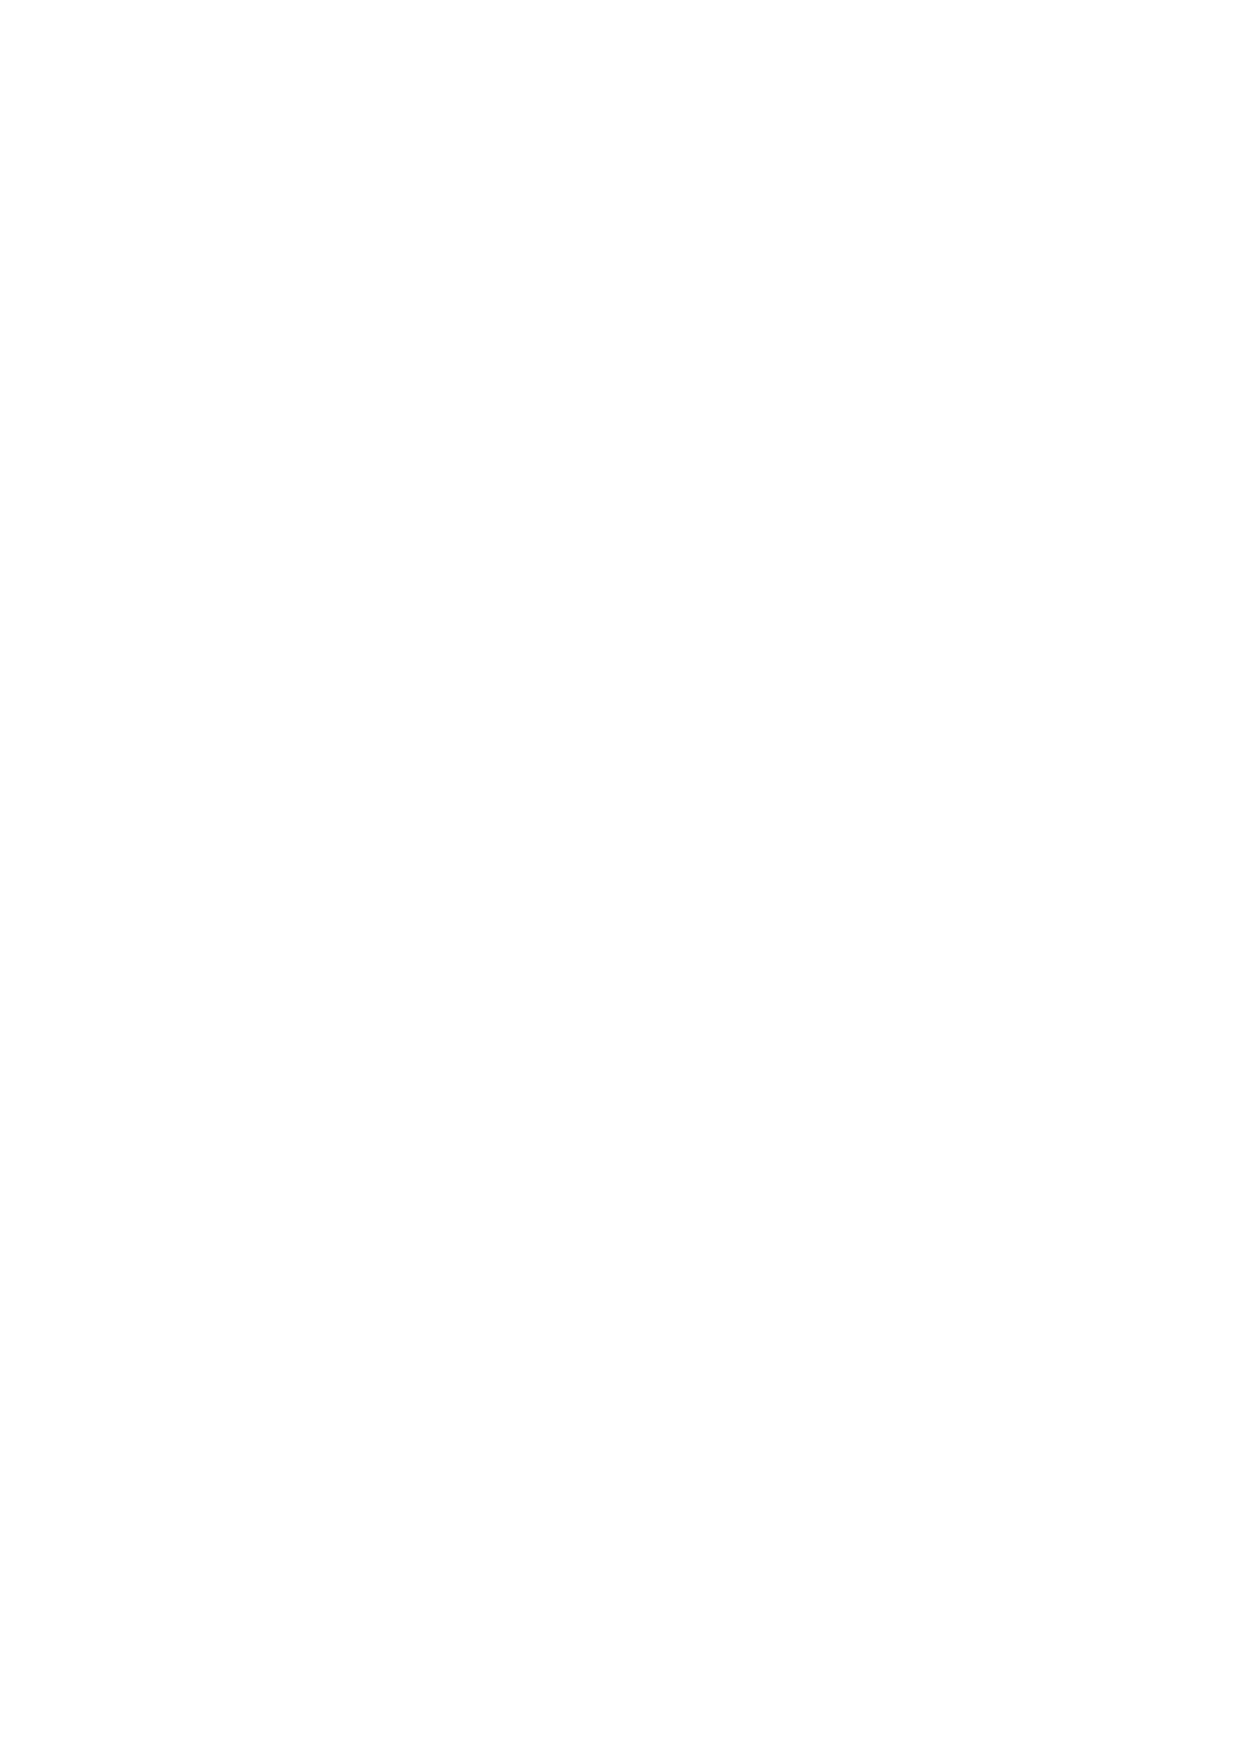
\includegraphics[width=\columnwidth]{./figs/ch4_tangent_prod}
			%\vspace*{-10cm}
			\resizebox{\columnwidth}{!}{\begin{tikzpicture}
[scale =2,>=stealth,point/.style = {draw, circle, fill = black, inner sep = 1pt},]

\def\rad{2}
\coordinate [point, label={above: $O$ }] (O) at (0, 2);
\draw (O) circle (\rad);
\node (P) at (-4,0)[point,label=below :$P$] {};
\node (C) at (0,0)[point,label=below :$C$] {};
\node (A) at (-1.92,1.45)[point,label=above left :$A$] {};
\node (B) at (1.2,3.6)[point,label=above right :$B$] {};
\draw (O)--(P);
\draw (P)--(C);
\draw (P)--(B);
%\draw (A)--(O);
%\draw (B)--(C);

\draw [thick,dashed](A)--(O);
\draw [thick,dashed](C)--(O);
\draw [thick,dashed](B)--(O);
%\tkzMarkRightAngle[size=.2](P,C,O);
%\tkzMarkAngle[size=.3](A,B,C);
%\tkzMarkAngle[size=.4](O,C,A);
%\tkzMarkAngle[size=.5](B,C,O);
%\tkzMarkAngle[size=.3](P,A,C);
%\tkzMarkAngle[size=.2](C,A,O);
%\tkzMarkAngle[size=.2](A,O,C);
%
\node [above] at (0.35,2.5){$r$};
\node [above] at (-0.9,1.7){$r$};
\node [above] at (0.1,1.0){$r$};
%\draw (-1.9,1) node{$\theta$};

%\draw (0.95,3.3) node{$\alpha$};
%\draw (-0.2,1.7) node{$2\alpha$};
%\draw (-0.2,0.5) node{$90-\alpha$};
%\draw (-1.4,1.4) node{$90-\alpha$};
%\draw (.1,.6) node{$\phi$};

\end{tikzpicture}}
		\end{center}
		\caption{$PA.PB = PC^2$.}
		\label{fig:tangent_secant}	
	\end{figure}
\solution Let $\vec{P} = \mbf{0}$.  Then, we have the following equations
\begin{align}
\label{eq:tan_sec_AB}
PA.PB &= \lambda \norm{\vec{A}}^2 \quad \because (\vec{B} = \lambda \vec{A})
\\
\norm{\vec{A}-\vec{O}}^2 &= \norm{\vec{B}-\vec{O}}^2 = \norm{\vec{C}-\vec{O}}^2 = r^2
\\
\norm{\vec{O}}^2-\norm{\vec{C}}^2 &=  r^2 \quad \triangle PCO\text{ is 
right angled}
\label{eq:tan_sec_boudh}
\end{align}
$\because$
\begin{align}
%\label{eq:tan_sec_AB}
%PA.PB &= \lambda \norm{\vec{A}}^2 \quad \because (\vec{B} = \lambda 
%\vec{A})
%\\
\norm{\vec{B}-\vec{O}}^2-\norm{\vec{A}-\vec{O}}^2   &=0,
\\
\brak{\lambda^2-1}\norm{\vec{A}}^2 - 2 \brak{\lambda-1}\vec{A}^T\vec{O} &= 
0
\\
\implies PA.PB = \lambda\norm{\vec{A}}^2 =  2 
\vec{A}^T\vec{O}-\norm{\vec{A}}^2 &
%\norm{\vec{C}-\vec{O}}^2 = r^2
%\\
%\norm{\vec{O}}^2-\norm{\vec{C}}^2 &=  r^2 \quad \triangle PCO\text{ is 
%right angled}
%\label{eq:tan_sec_boudh}
\label{eq:tan_sec_first}
\end{align}
after substituting from \eqref{eq:tan_sec_AB} and simplifying. From 
\eqref{eq:tan_sec_boudh},
\begin{align}
\norm{\vec{A}-\vec{O}}^2 = \norm{\vec{O}}^2-\norm{\vec{C}}^2  &= r^2
\\
\implies 2 \vec{A}^T\vec{O}-\norm{\vec{A}}^2   = \norm{\vec{C}}^2 = PC^2&
\label{eq:tan_sec_second}
\end{align}
From \eqref{eq:tan_sec_first} and \eqref{eq:tan_sec_second},
\begin{align}
PA.PB = PC^2
\end{align}

\item In Fig. \ref{fig:chords} show that $PA.PB = PC.PD$.
\begin{figure}[!ht]
	\begin{center}
		
		%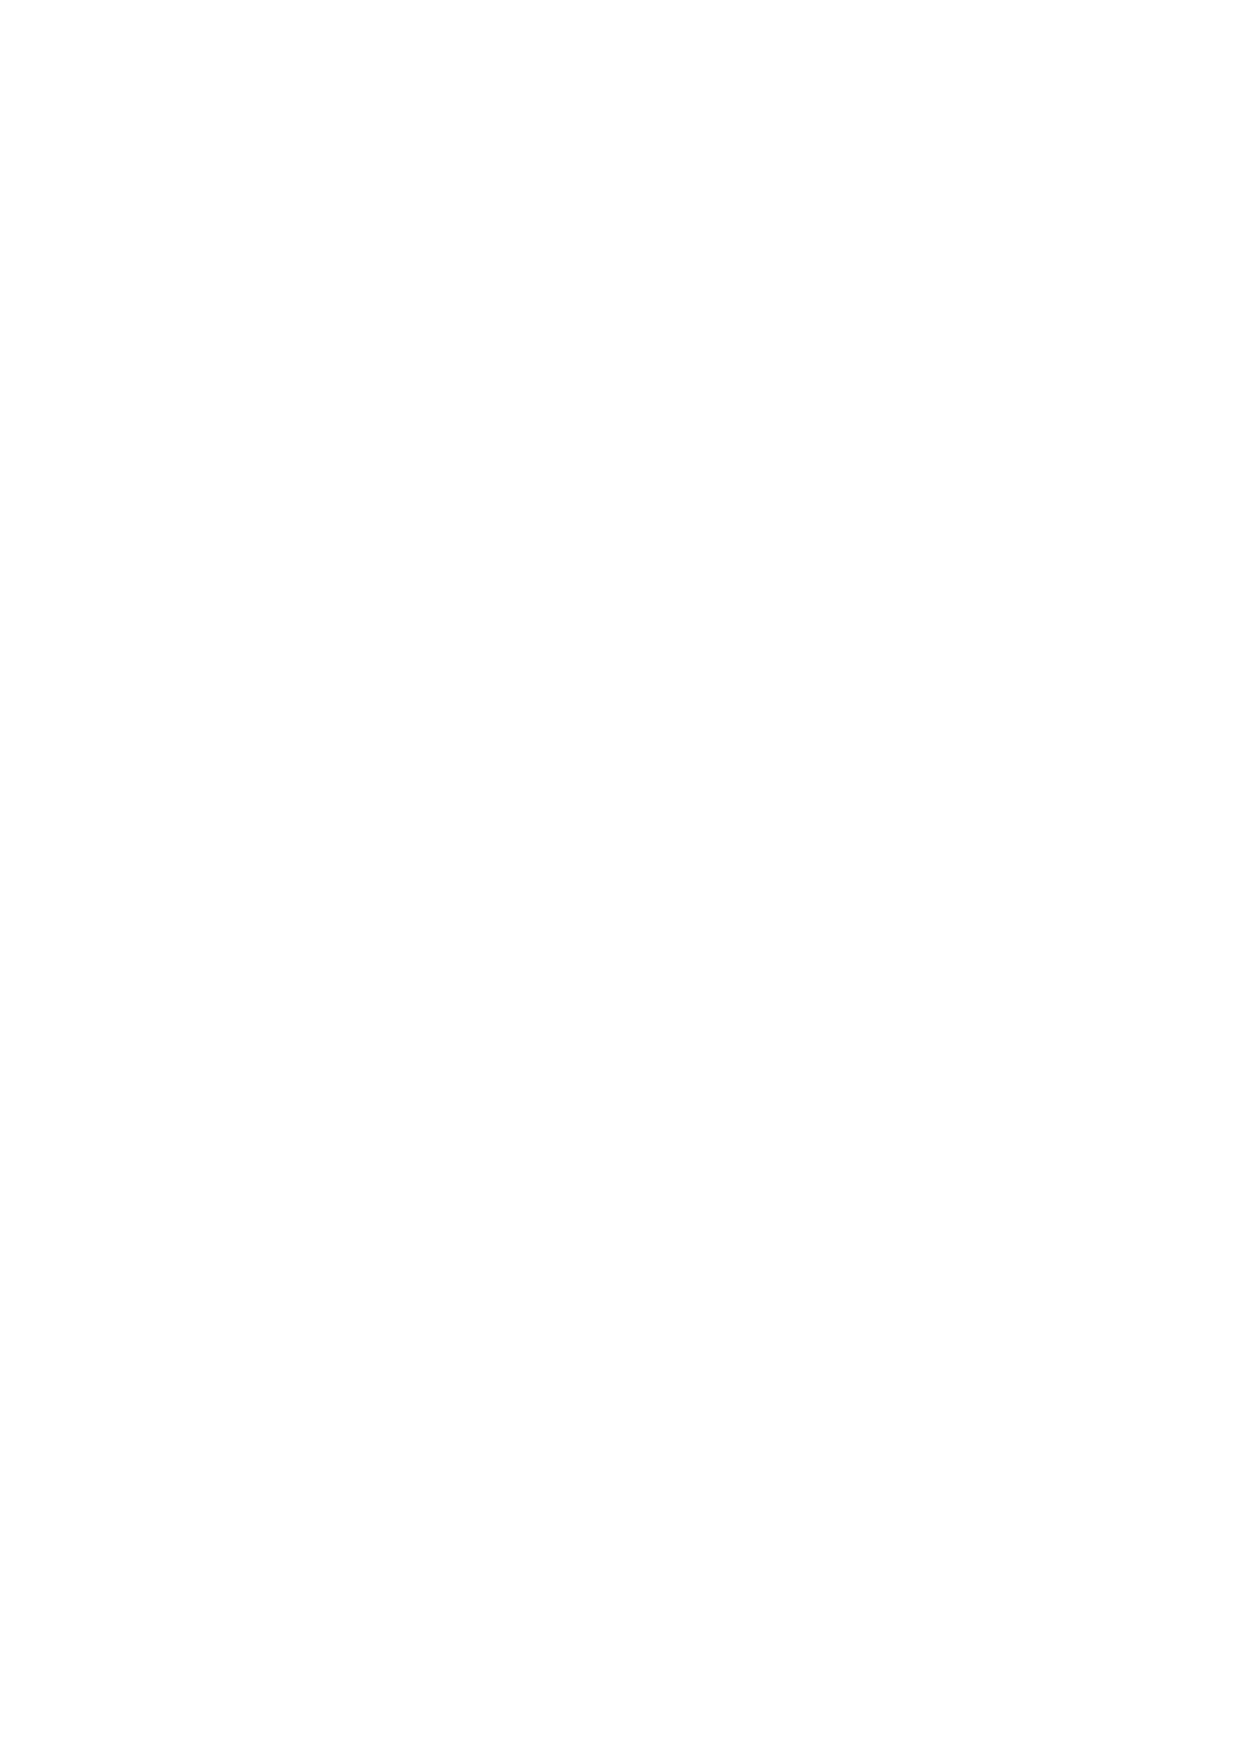
\includegraphics[width=\columnwidth]{./figs/ch3_angle_bisector}
		%\vspace*{-10cm}
		\resizebox{\columnwidth}{!}{\begin{tikzpicture}
[scale=2,>=stealth,point/.style={draw,circle,fill = black,inner sep=0.5pt},]
%\node (D) at (0, 0)[point,label=below :$D$] {};
\node (B) at (-2, -2)[point,label=below left :$C$]{};
\node (A) at (1, 3)[point,label=above:$A$]{};
\node (C) at (4, -1)[point,label=below right:$B$]{};
%\coordinate [point, label={above : $O$ }] (I) at  (1.147, 1.143);
\node (O) at (0.7962963,-0.27777778)[point,label=above:$O$]{};
\node (D) at (  3.64041158, 1.36427295)[point,label=below:$D$]{};
\node (P) at ( 2.66371481, 0.78171359)[point,label=right:$P$]{};
%\node (x1) at (0.601,-1.357)[point,label=left:$x_1$]{};
%\node (x2) at (2.15,-1.1)[point,label=right:$x_2$]{};
%\node (temp) at ($(O)!0.5!(D)$)[label=right:$r$]{};
%\node (D) at (2.424,1.1)[point,label=above right:$D$]{};
%\node (E) at (1.1, 1.9)[point,label=above right:$E$]{};
%\node (F) at (-1.1, 1.9)[point,label=above left:$F$]{};
\def\rad{3.284101453883}
\draw (O) circle (\rad);

%\draw (D)--(O);
%\draw (A)--(B);
\draw (B)--(D);
\draw (A)--(C);
%\draw (C)--(D);
%\draw [thick,dashed] (x1) -- (x2);
%\draw [thick,dashed] (O) -- (E);
%\draw [thick,dashed] (O) -- (F);
%\draw (B)--(O);
%\draw (C)--(O);

%\tkzMarkRightAngle[size=.2](A,D,C)
%\tkzMarkRightAngle[size=.15](B,F,O);
%\tkzMarkRightAngle[size=.15](C,E,O);
%\tkzMarkAngle[size=.4](D,B,O);
%\tkzMarkAngle[size=.35](O,B,F);
%\tkzMarkAngle[size=.54](E,C,O);
%\tkzMarkAngle[size=.5](E,C,O);
%\tkzMarkAngle[size=.6](O,C,D);
%\tkzMarkAngle[size=.65](O,C,D);

\end{tikzpicture}}
	\end{center}
	\caption{Chords of a circle}
	\label{fig:chords}	
\end{figure}
\\
\solution Let $\vec{P} = \mbf{0}$.  We then have the following equations
\begin{align}
\begin{split}
\vec{B} &= k_1 \vec{A}, k_1 = \frac{PB}{PA}
\\
\vec{D} &= k_2 \vec{C}, k_2 = \frac{PD}{PC}
\end{split}
\label{eq:chords_ratio}
\\
\begin{split}
\norm{\vec{A}-\vec{O}}^2 &= \norm{\vec{B}-\vec{O}}^2 
\\
= \norm{\vec{C}-\vec{O}}^2 &= \norm{\vec{D}-\vec{O}}^2 = r^2
\end{split}
\label{eq:chords_points}
\end{align}
%
where $r$ is the radius of the circle and $\vec{O}$ is the centre. From \eqref{eq:chords_points},
\begin{align}
&\norm{\vec{A}-\vec{O}}^2 = \norm{\vec{B}-\vec{O}}^2
\\
\implies &\norm{\vec{A}-\vec{O}}^2 = \norm{k\vec{A}-\vec{O}}^2 \quad(\text{from \eqref{eq:chords_ratio}})
\end{align}
%
which can be simplified to obtain
\begin{align}
k_1\norm{\vec{A}}^2 = 2\vec{A}^T\vec{O}-\norm{\vec{A}}^2
\label{eq:chords_Anorm}
\end{align}
Similarly,
\begin{align}
k_2\norm{\vec{C}}^2 = 2\vec{C}^T\vec{O}-\norm{\vec{C}}^2
\label{eq:chords_Cnorm}
\end{align}
%
From \eqref{eq:chords_points}, we also obtain
\begin{align}
\norm{\vec{A}-\vec{O}}^2 
= \norm{\vec{C}-\vec{O}}^2 
\\
\implies 2\vec{A}^T\vec{O}-\norm{\vec{A}}^2 = 2\vec{C}^T\vec{O}-\norm{\vec{C}}^2
\label{eq:chords_ACnorm}
\end{align}
%
after simplification. Using this result in \eqref{eq:chords_Anorm} and \eqref{eq:chords_Cnorm},
\begin{align}
k_1\norm{\vec{A}}^2 = k_2\norm{\vec{C}}^2
\\
\implies \norm{\vec{A}}\, \norm{\vec{B}}=\norm{\vec{C}}\,\norm{\vec{D}}
\end{align}
which completes the proof.

\end{enumerate}
\section{Parabola}
\begin{enumerate}[label=\thesection.\arabic*
,ref=\thesection.\theenumi]
\item Express 
\begin{align}
y_2 = y_1^2
\label{eq:parab}
\end{align}
as a matrix equation.
\\
\solution  \eqref{eq:parab} can be expressed as
\begin{align}
\vec{y}^T\vec{W}\vec{y}+2\vec{g}^T\vec{y} = 0
\label{eq:parab_mat}
\end{align}
%
where 
\begin{align}
\vec{W} = \myvec{1 & 0 \\ 0 & 0} 
,
\vec{g} &= -\frac{1}{2}\myvec{0 \\ 1}
\label{eq:parab_coeffs}
\end{align}
%
\item Given 
\begin{align}
\vec{x}^T\vec{V}\vec{x}+2\vec{u}^T\vec{x}+ F = 0,
\label{eq:parab_gen}
\end{align}
where 
\begin{align}
\vec{V}=\vec{V}^T, \det(\vec{V}) = 0,
\label{eq:parab_vcond}
\end{align}
%
and $\vec{P}, \vec{c}$ such that
\begin{align}
\vec{x} = \vec{P}\vec{y}+\vec{c}.
\label{eq:parab_affine}
\end{align}
Show that
\begin{align}
\begin{split}
\vec{W} &= \vec{P}^T\vec{V}\vec{P}
\\
\vec{g} &= \vec{P}^T\brak{\vec{V}\vec{c}+\vec{u}}
\\
F+ \vec{c}^T\vec{V}\vec{c} + 2\vec{u}^T\vec{c}&= 0
\end{split}
\label{eq:parab_parmas}
\end{align}

\solution Substituting \eqref{eq:parab_affine} in \eqref{eq:parab_gen},
\begin{align}
\brak{\vec{P}\vec{y}+\vec{c}}^T\vec{V}\brak{\vec{P}\vec{y}+\vec{c}}+2\vec{u}^T\brak{\vec{P}\vec{y}+\vec{c}}+ F = 0, 
\end{align}
which can be expressed as
\begin{multline}
\implies \vec{y}^T\vec{P}^T\vec{V}\vec{P}\vec{y}+2\brak{\vec{V}\vec{c}+\vec{u}}^T\vec{P}\vec{y}
\\
+ F+ \vec{c}^T\vec{V}\vec{c} + 2\vec{u}^T\vec{c} = 0
\label{eq:parab_simp}
\end{multline}
%
Comparing \eqref{eq:parab_simp} with \eqref{eq:parab_mat} \eqref{eq:parab_parmas} is obtained.
%
\item Show that there exists a $\vec{P}$ such that 
\begin{align}
\vec{P}^T\vec{P} = \vec{I}
\end{align}
%
Find $\vec{P}$ using
\begin{align}
\vec{W} = \vec{P}^T\vec{V}\vec{P}
\end{align}
\item Find $\vec{c}$ from \eqref{eq:parab_parmas}.
\\
\solution 
\begin{align}
\because \vec{g} &= \vec{P}^T\brak{\vec{V}\vec{c}+\vec{u}},
\\
\vec{V}\vec{c}&= \vec{P}\vec{g} - \vec{u}
\\
\implies \vec{c}^T\vec{V}\vec{c} &= \vec{c}^T\brak{\vec{P}\vec{g} - \vec{u}} = -F- 2\vec{u}^T\vec{c}
\end{align}
%
resulting in the matrix equation
\begin{align}
\myvec{\vec{V}\\ \brak{\vec{P}\vec{g} + \vec{u}}^T}\vec{c}&= \myvec{\vec{P}\vec{g} - \vec{u}\\ -F}
\end{align}
%
for computing $\vec{c}$.
\end{enumerate}


\end{document}
